\documentclass{sig-alternate-10pt-CoNEXT}
%\usepackage[small,bf]{caption}
\usepackage{caption}
\usepackage{subfig}
\usepackage{epstopdf}
\usepackage{color}
\usepackage[normalem]{ulem}
\usepackage{amsmath,amssymb}
\pagenumbering{arabic}
\setlength{\jot}{10pt} 
\renewcommand{\floatpagefraction}{0.8}

\usepackage{url}
%% Define a new 'leo' style for the package.
\makeatletter
\def\url@leostyle{%
  \@ifundefined{selectfont}{\def\UrlFont{\sf}}{\def\UrlFont{\normalsize\ttfamily}}}
\makeatother
%% Now actually use the newly defined style.
\urlstyle{leo}

\hyphenation{Wi-Gem amen-able mar-ginal}
\begin{document}

% --- Author Metadata here ---
%\conferenceinfo{WOODSTOCK}{'97 El Paso, Texas USA}
%\CopyrightYear{2007} % Allows default copyright year (200X) to be over-ridden - IF NEED BE.
% ACM CoNEXT 2008: the following needs to be over-ridden to include the
% right copyright info
%\crdata{0-12345-67-8/90/01}  % Allows default copyright data (0-89791-88-6/97/05) to be over-ridden - IF NEED BE.
% --- End of Author Metadata ---

\pagestyle{empty}
\title{WiGEM : A Learning-Based Approach for Indoor Localization}
%\subtitle{[  Paper Id : 1569469851. Number of Pages : 12 ]}
%
% You need the command \numberofauthors to handle the 'placement
% and alignment' of the authors beneath the title.
%
% For aesthetic reasons, we recommend 'three authors at a time'
% i.e. three 'name/affiliation blocks' be placed beneath the title.
%
% NOTE: You are NOT restricted in how many 'rows' of
% "name/affiliations" may appear. We just ask that you restrict
% the number of 'columns' to three.
%
% Because of the available 'opening page real-estate'
% we ask you to refrain from putting more than six authors
% (two rows with three columns) beneath the article title.
% More than six makes the first-page appear very cluttered indeed.
%
% Use the \alignauthor commands to handle the names
% and affiliations for an 'aesthetic maximum' of six authors.
% Add names, affiliations, addresses for
% the seventh etc. author(s) as the argument for the
% \additionalauthors command.
% These 'additional authors' will be output/set for you
% without further effort on your part as the last section in
% the body of your article BEFORE References or any Appendices.
\numberofauthors{1} %  in this sample file, there are a *total*
% of EIGHT authors. SIX appear on the 'first-page' (for formatting
% reasons) and the remaining two appear in the \additionalauthors section.
%
\author{
% You can go ahead and credit any number of authors here,
% e.g. one 'row of three' or two rows (consisting of one row of three
% and a second row of one, two or three).
%
% The command \alignauthor (no curly braces needed) should
% precede each author name, affiliation/snail-mail address and
% e-mail address. Additionally, tag each line of
% affiliation/address with \affaddr, and tag the
% e-mail address with \email.
%
% 1st. author
\alignauthor
Abhishek Goswami, Luis E. Ortiz, Samir R. Das\\
       \affaddr{Computer Science Department, Stony Brook University, Stony Brook, New York 11794, USA}\\
%       \affaddr{Stony Brook University}\\
%       \affaddr{Stony Brook, New York 11794, USA}\\
       \email{agoswami,leortiz,samir@cs.stonybrook.edu}
% 2nd. author
%\alignauthor
%Luis Ortiz
%       \affaddr{Computer Science Department}\\
%       \affaddr{Stony Brook University}\\
%       \email{leortiz@cs.stonybrook.edu}
%% 3rd. author
%\alignauthor 
%Samir R. Das
%       \affaddr{Computer Science}\\
%       \affaddr{Stony Brook University}\\
%       \email{samir@cs.stonybrook.edu}
}

%\date{03 June 2011}

\maketitle
\begin{abstract}
We consider the problem of localizing a wireless client in an
indoor environment based on the signal strength of its transmitted
packets as received on stationary sniffers or access points.
Several state-of-the-art indoor localization techniques have the
drawback that they rely extensively on a labor-intensive`training' phase that does not scale 
well.  Use of unmodeled hardware with heterogeneous
power levels further reduces the accuracy of these
techniques.

We propose a `learning-based' approach, WiGEM, where the received signal
strength is modeled as a Gaussian Mixture Model (GMM). Expectation
Maximization (EM) is used to learn the maximum likelihood estimates of 
the model parameters. 
This approach enables us to localize a transmitting device based on the 
\textit{maximum a posteriori} estimate. The key insight is to use the physics of wireless propagation, 
and exploit the signal strength constraints that exist for different transmit power levels. 
The learning approach not only avoids the 
labor-intensive
training, but also makes the location estimates considerably robust in the face of heterogeneity and 
various time
varying phenomena.  We present evaluations on two different
indoor testbeds with multiple WiFi devices. We demonstrate that WiGEM's
accuracy is at par with or better than state-of-the-art techniques but
without requiring any training.
\end{abstract}

\section{Introduction}
\label{sec:introduction}

Over the past decade, the increasing use of wireless networking has fueled the 
use of wireless links to localize wireless clients in indoor spaces. This issue
is increasingly finding attention both from research and business communities 
because a perfect, general-purpose solution such as outdoor GPS has been elusive. Close scrutiny 
of available techniques reveal that more successful techniques require a substantial
`pre-deployment' effort by way of creating RF maps, for example. 
Technically, this is equivalent
to `training'. Fine grain RF map creation makes localization 
more accurate, but requires proportionately more effort.
On the other hand, any RF map is inherently device specific.
\emph{This pre-deployment burden that lacks generality
has made these localization techniques less appealing in practice.}  This paper develops a new machine-learning based localization algorithm, WiGEM,
that removes these limitations. 

%The received signal strength (RSS) based techniques are the most popular as commodity wireless devices are all capable of measuring RSS. 

Over time, two general localization approaches have emerged 
in literature -- (i) client-based approach~\cite{Haeberlen:2004:PRL:1023720.1023728, Gwon:2004:ECC:1023783.1023786, Youssef:2008:HLD:1399551.1399558, Chintalapudi:2010:ILW:1859995.1860016, Ladd:2002:RLS:570645.570674, Youssef:2003:WLD:826025.826335} and (ii)  infrastructure-based approach~\cite{Moraes:2006:CWL:1164783.1164799, Lim:2010:ZIL:1741400.1741464, Tao:2003:WLL:941311.941314, Krishnan04asystem}. In the client-based approach, the client device measures the RSS (received signal strength) as seen by it from various APs (access points). This information is used to localize the client. In the infrastructure-based approach, the network administrator can use simple sniffing devices (or APs doubling as sniffers) to monitor clients and record RSS from the client transmissions.  This sniffed RSS is used to localize the client. The infrastructure-based approach is more attractive for large scale deployment, because
any arbitrary client without any specific installed application can still localize itself
with the assistance of the infrastructure. It is also easier to deploy, manage and maintain. 

In the discussion that follows, we specifically focus on WiFi-based localization using
an infrastructure-based approach. WiFi is chosen because of the popularity of WiFi devices and WiFi-based WLAN systems. But the technique we develop is not specific to any link layer technology. At this point we also make a distinction between `learning' and `training'. By `learning' we actually mean unsupervised learning, whereby we automatically try to estimate our model parameters from unlabeled data. On the other hand, `training' is akin
to supervised learning that in our scenario leads to substantial limitations as discussed next.


%
%alluring for large-scale deployments, especially if building and maintaining the model can be automated. Moreover, such techniques perform location estimation without requiring hardware and/or software changes on the client device, which make them particularly attractive.
%
%
%
%Recent research has recognized this issue; however the proposed technique is not universally applicable~\cite{}. The goal of our work 
%to develop a unsupervised learning technique that works without any training
%
%the need for location-aware pervasive computing applications in indoor environments. Traditional GPS-based techniques have problems working indoor which make them unattractive for such fine-grained indoor localization. On the other hand, indoor wireless LAN (WLAN) technologies, which have been enthusiastically and widely adopted in enterprises and homes, give us interesting features like Received Signal Strength(RSS), Angle of Arrival(AoA) etc for robust location estimation. Received signal strength (RSS) is particularly interesting because current commercial hardware can be used to extract the signal strength of wireless frames being transmitted by a Wi-Fi device. 
%
%Several techniques [x, y, x] have demonstrated the viability of using the RSS metric for location estimation.   It is interesting to note here that most of these location-estimation systems can essentially be categorized in two distinct ways : a client-based approach [p, q, r] and an infrastructure-based approach [a, b, c]. In the client-based approach, the client device measures the signal strength as seen by it from various AP(Access Point). This information is used to locate the client. In the infrastructure-based approach, the network administrator can use simple sniffing devices (or APs masquerading as sniffers) to monitor clients and extract the RSS from the tx-client.  This sniffed information is used to locate the client. Considering ease of management, provisioning, security, deployment,  maintenance etc, the infrastructure-based model seems alluring for large-scale deployments, especially if building and maintaining the model can be automated. Moreover, such techniques perform location estimation without requiring hardware and/or software changes on the client device, which make them particularly attractive.
%

\subsection{Limitations of Training}
\label{subsec:limitationsoftraining}

In the existing indoor WiFi localization solutions, the first phase is a pre-deployment `offline phase' or training phase aimed at building detailed RF maps or RF propagation models based on a survey of the target area. The second phase is the `online phase', where a localization algorithm is used to provide a location estimate for an observed set of RSS measurements from the mobile device being localized. There are three major drawbacks of this general approach. 
\begin{enumerate}
\item
The device used during the `offline phase' may differ from the target device in the `online phase'. Unmodeled hardware devices operating at different transmit power levels can introduce significant variations in the signal patterns between the training device and the target device. This adversely affects the accuracy of location estimation \cite{Tsui:2009:ULS:1741410.1741596}. Experiments described later in this paper indicate how hardware variations between four common commodity WiFi devices can significantly degrade the accuracy of two commonly used localization algorithms. 
\item
The `offline phase' itself involves labor-intensive sampling of signal strength values at discrete locations in the target space. Again, experiments show that location accuracy depends significantly on the granularity of the training locations. If the training locations are sparse, the location estimates become substantially poorer.
\item
Static models built during the `offline phase' cannot counter time varying phenomena like movement of people, changing occupancy and surroundings etc. Most 
`killer' applications of indoor localization would be in large shopping malls, airports, 
convention centers etc., where such changes would be routine. 
On the other hand, due to the reason 2 above, such models are difficult to update regularly. 
\end{enumerate}

\subsection{Approach}

We propose WiGEM, a novel {\bf Wi}reless
localization algorithm that uses the {\bf G}aussian Mixture Model (GMM) and employs {\bf E}xpectation 
{\bf M}aximization (EM) to estimate the model parameters. 
The model is initialized 
using  a standard radio propagation model~\cite{Rappaport:2001:WCP:559977, Molkdar91} 
and typical constraints that exist between the received signal strengths for different transmit 
power levels at the same 
location.

WiGEM leverages the infrastructure based approach 
while eliminating any `pre-deployment' effort. Packet transmissions made by a client are received on stationary sniffers 
(or APs doubling as sniffers) that extract the RSS and MAC id of the target client and report this information to a 
central localization server. Using this information, WiGEM builds a model for the target device and provides 
a location estimate. The estimate can be made available to the client via a simple web-based
application,  for example, depending on the intended application. But this is not a part
of the current work. 



WiGEM provides several key benefits by eliminating the `offline phase'. First, building a model for each target device effectively addresses the hardware variance problem. Thus, WiGEM can be used across heterogeneous devices, each operating at different power levels.  Second, zero `pre-deployment' effort makes WiGEM particularly attractive for large indoor spaces. Third, WiGEM is a purely online algorithm: the model parameters get updated and modified based on real-time RSS observations. As such, WiGEM is able to adapt to dynamic changes in the target space.

The remainder of the paper is organized as follows. In Section~\ref{sec:relatedwork}, we survey related work in Indoor Localization. In Section~\ref{sec:problemformulation} we introduce WiGMM, the modeling approach we use to localize a target device, and discuss the parameters of the model. In Section~\ref{sec:emalgorithm} we discuss the EM algorithm, which is used to estimate the parameters of our model. Section~\ref{sec:experimentmethodology} provides details on the experiment methodology and Section~\ref{sec:evaluation} presents the experimental results obtained from two different testbeds. In Section~\ref{sec:discussion} we discuss WiGEM and identify items for future work. Finally, we present our conclusions in Section~\ref{sec:conclusions}.

% \textbf{Our results of deploying GEM in two different office buildings are promising. We specifically note that when measurements made using one device are used to localize a different device,  GEM is seen to perform better that RF signal map based techniques like RADAR[x] and Probabilistic[y]
% }
\section{Related Work}
\label{sec:relatedwork}

In this section we provide a brief overview of some
of the fundamental techniques in the field of indoor wireless 
localization. In passing, we also point out their limitations
with respect to the proposed WiGEM technique. \\

%Over the past two decades, this field has seen tremendous push, both from the research community and from industrial circles. The advent of pervasive and mobile computing has fueled tremendous interest in this field in recent years.  \\

\noindent {\bf Calibration-free techniques:} An indoor path-loss propagation model essentially forms the bedrock for these techniques. In RADAR, Bahl {\it et al} \cite{Bahl00radar:an} 
provide a indoor radio propagation model to calculate RSS at various locations in the building based on distance, number of walls etc. The nearest neighbor in signal space (NNSS) metric is then used to estimate the location of the  mobile user by matching the observed RSS to the theoretically computed signal strength values at these locations. In \cite{Moraes:2006:CWL:1164783.1164799, Lim:2010:ZIL:1741400.1741464} the authors describe sniffer based techniques for localization based on propagation models. Moraes {\it et al} \cite{Moraes:2006:CWL:1164783.1164799} use a naive propagation model to generate a `radio propagation map' (RPM) at each sniffer. They use RSS measurements between the sniffers and a `reference AP' (APRef) to reconstruct the RPM, either periodically or when there are significant variations in the RSS. A probabilistic model is then used to compute a location estimate.  Lim {\it et al}~\cite{Lim:2010:ZIL:1741400.1741464} consider online measurements of RSS between 802.11 APs and between a client and its neighboring APs, to create a mapping between the RSS measure and the actual geographic distance. TIX~\cite{Gwon:2004:ECC:1023783.1023786} uses a similar setting whereby inter-AP and client-AP RSS measurements are used to perform linear interpolation for estimating the RSS at distinct locations in the target space. Madigan {\it et al}~\cite{Madigan05bayesianindoor} propose a client-based scheme that uses a Bayesian hierarchical graphical model. By making the assumption that different access points behave similarly, they develop a model which avoids the need to know the location of the training points. {\it While most of these schemes are designed to be responsive to real time changes in the environmental dynamics of the target space, none of them model variations in client hardware and transmission power, factors which can significantly degrade the accuracy estimates of RSS based WiFi localization schemes.} \\

\noindent {\bf Techniques that build RF signal maps:} Several client-based schemes and infrastructure-based schemes rely on RF signal maps for localization.  The basic approach is to have a pre-deployment `offline phase' or training phase aimed at building detailed RF maps or RF propagation models based on a survey of the target area. The client device is then localized by matching the observed RSS against the signal map. RADAR-empirical \cite{Bahl00radar:an} was one of the first RF-based schemes to use this model. In recent years, a number of probabilistic techniques \cite{Youssef:2008:HLD:1399551.1399558, Ladd:2002:RLS:570645.570674, Haeberlen:2004:PRL:1023720.1023728} have been proposed to enhance the robustness of localization. For the probabilistic techniques, the `offline phase' corresponds to the construction of conditional  probability distributions that map signal intensities to locations on a map.  %Thus, we first build up a {\it signal map} database for the area being covered. 
During the location determination phase, given a real-time RSS signature,  a probabilistic inference algorithm is used to select the most likely location from all possible locations in the target space. As mentioned in Section~\ref{subsec:limitationsoftraining}, \emph{these techniques require considerable `pre-deployment' training effort, are difficult to maintain and update with changing dynamics in the target space and are inherently susceptible to the hardware variance problem~\cite{Tsui:2009:ULS:1741410.1741596}. }\\


\noindent{\bf Prior work on hardware variance:} Tsui {\it et al}~\cite{Tsui:2009:ULS:1741410.1741596} observe that hardware variance can significantly degrade the positional accuracy of RSS-based Wi-Fi localization systems. In fact, they note that the hardware variance problem is not limited to differences in the WiFi chipsets used by training and tracking devices, but also occurs when the same Wi-Fi chipsets are connected to different antenna types and/or packaged in different encapsulation materials. The authors introduce an intermediate `online adjustment' phase where they use unsupervised learning to construct a signal transformation function between the training device and a new target device. Prior work on hardware variance \cite{Haeberlen:2004:PRL:1023720.1023728} observe a linear relationship between the RSS mappings of several commodity Wi-Fi cards and suggest a manual calibration effort to identify this relationship between different cards. {\it The ever-increasing number of WiFi chipsets, antennas and encapsulating materials make this manual adjustment effort impractical in real-world deployments}. 

Tao {\it et al}~\cite{Tao:2003:WLL:941311.941314} have an interesting take on unmodeled hardware and transmission power variations.  They observe that RSS is linearly proportional to transmission power. Based on the difference in signal strength between every pair of sniffers, they suggest a weighted heuristic to give a location estimate for a target RSS fingerprint.\\

\noindent{\bf WiGEM compared to prior work:} The major contribution of this work is to develop an algorithm, WiGEM, that eliminates the expensive `training' phase. 
While a similar attempt has also been made in a recent work~\cite{Chintalapudi:2010:ILW:1859995.1860016}, this technique depends on the availability of GPS feed in some indoor
locations, more the better. WiGEM does not depend on availability of GPS. 
%
WiGEM can adapt to variations in transmit power across heterogeneous devices, which makes it particularly suitable for infrastructure-based localization schemes. The algorithm also `learns on the go' and thus can factor in real-time changes in the environmental dynamics of the target space. 

%\input{wireless}

\section{Problem Formulation}
\label{sec:problemformulation}

Assume that the target space is discretized into $J$ locations. 
This can be of any level of granularity 
depending on the desired accuracy. Finer granularity does increase computational load, but does not seem to be a bottleneck. There are a set of sniffers or APs doubling as sniffers (a larger number is expected to improve accuracy) that report a vector of RSSs from a target device to be localized to a server that performs the necessary computation. The target device can be static or mobile. In fact, mobility tends to improve performance (more on this later). The location of the sniffers themselves are assumed to be known with respect to which the $J$ locations
are specified. No prior wireless measurements are needed.
%providing our approach with a significant leverage. 

\subsection{Using Gaussian Mixture Model}
We use the well-known idea of {\em mixture models} in statistics. The idea is to first make a very general assumption that the target could be in any of the $J$ possible locations with varying probabilities. Each of these possibilities can potentially generate a distribution of RSSs
at the set of sniffers. Now, given the vector of RSSs sniffed at the set of sniffers, the problem is to estimate the most likely target 
location out of the $J$ possibilities that could have generated that vector of RSSs. Since 
the same device at the same location but with a different transmit power can generate different distributions of RSSs, an additional subtlety we handle is that the
most likely power level (actually an abstract sense of it) is also
determined as a part of the process. This subtle addition makes the
method adaptive for different devices having their own default power
levels for wireless transmission.

\begin{figure} 
\centering
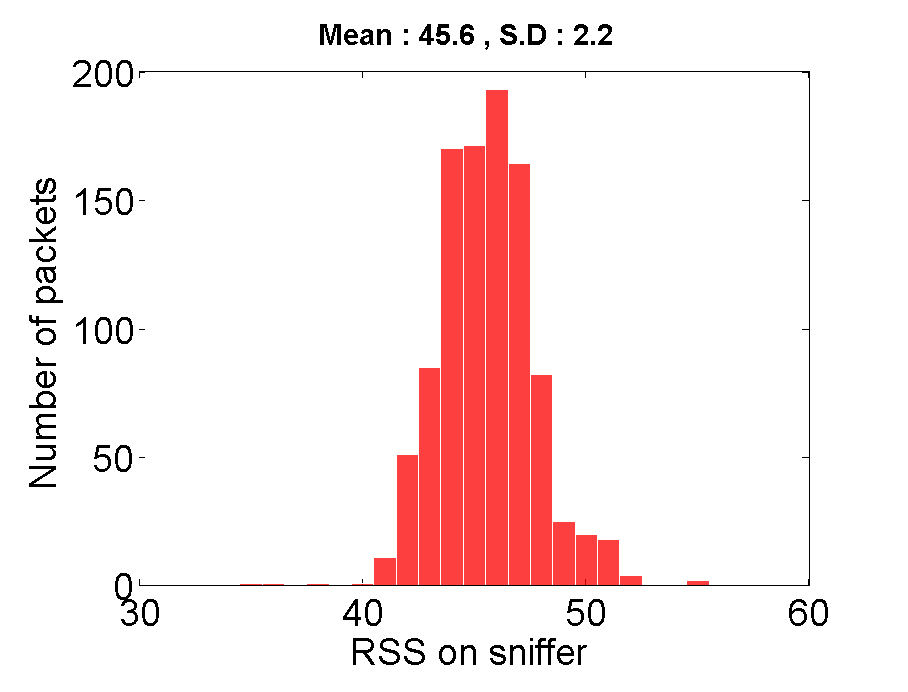
\epsfig{file=Figs4Paper/NewGaussian/distr7.eps, height=1.25in, width=1.6in} 
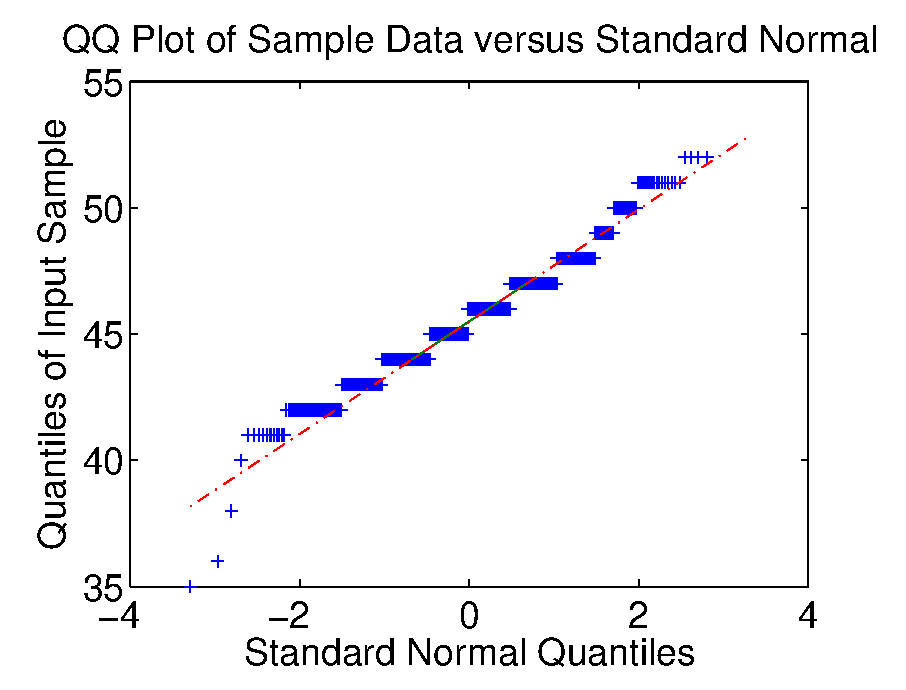
\epsfig{file=Figs4Paper/NewGaussian/qqplot2.eps, height=1.25in, width=1.6in}
\caption{The distribution of RSS observed on a sniffer.}
\label{fig:distribution}
\end{figure}

Before a more formal presentation, a key assumption we must make upfront
is that the distribution of RSS at a sniffer (more specifically an indicator representing RSS, commonly known as RSSI) is Gaussian
given the target device is stationary at a location and transmitting at
a fixed power level. The Gaussian assumption is not uncommon in wireless link modeling~\cite{Haeberlen:2004:PRL:1023720.1023728, Moraes:2006:CWL:1164783.1164799, Tao:2003:WLL:941311.941314}. In fact, the log-normal shadowing model~\cite{Rappaport:2001:WCP:559977} is widely used albeit in a slightly different context. To lend confidence to this assumption on our specific hardware setup, we have performed a set of measurements using the same sniffer and target device hardware used in later experiments. 
Figure~\ref{fig:distribution} shows the measured
RSSI distribution observed on a sniffer in our testbed 
for a stationary client transmitting at a fixed power level. The quality of the Gaussian fit for this distribution is also shown. The fit is very good. 

The Gaussian assumption makes our approach amenable to well-known machine learning tools. Now,
the distribution of the RSSs on the sniffers can be represented by the \emph{Gaussian Mixture Model} or GMM~\cite{Reynolds, Bishop:2006:PRM:1162264} --  a simple linear superposition of Gaussian components. 
Nothing is known a priori about the nature of these Gaussian
and in what proportion they are mixed. They are modeled in terms of discrete latent variables. We describe the modeling approach below.  

\subsection{Latent Variables for Target Locations and Power Levels}
\label{subsec:latentvariablesfortargetlocationsandpowerlevels}

Assume that a $J$-dimensional binary random variable {\bf x} representing possible target locations. $\mathbf{x}$ has a 1-of-$J$ representation in which a particular element $x_{j}$ is equal to one and all other elements are equal to $0$. The values of $x_{j}$ therefore satisfy $x_{j} \in$ \{0,1\} and $\sum_{j} x_{j} = 1$. Thus, there are $J$ possible states for the vector $\mathbf{x}$.

The probability distribution over $\mathbf{x}$ can be specified as a multinomial 
\begin{align}
 p(x_{j} = 1) = \upsilon_{j},
\end{align}
where the parameters $\{\upsilon_{j}\}$ must satisfy
\begin{align}
0 \le \upsilon_{j} \le 1 \ \text{and} \ \sum_{j=1}^{J} \upsilon_{j} = 1.
\end{align}

Similarly, assume that a $K$-dimensional binary random variable $\mathbf{z}$ representing Power Levels. $\mathbf{z}$ has a 1-of-$K$ representation in which a particular element $z_{k}$ is equal to 1 and all other elements are equal to 0. The values of $z_{k}$ therefore satisfy $z_{k} \in$ \{0,1\} and $\sum_{k} z_{k} = 1$. Vector {\bf z} has $K$ possible states.

The distribution over $\mathbf{z}$ is specified as a multinomial 
\begin{align}
p(z_{k} = 1) = \tau_{k},
\end{align}
where the parameters $\{\tau_{k}\}$ must satisfy
\begin{align}
0 \le \tau_{k} \le 1 \ \text{and} \  \sum_{k=1}^{K} \tau_{k} = 1.
\end{align}


\begin{figure} [h!]
\centering
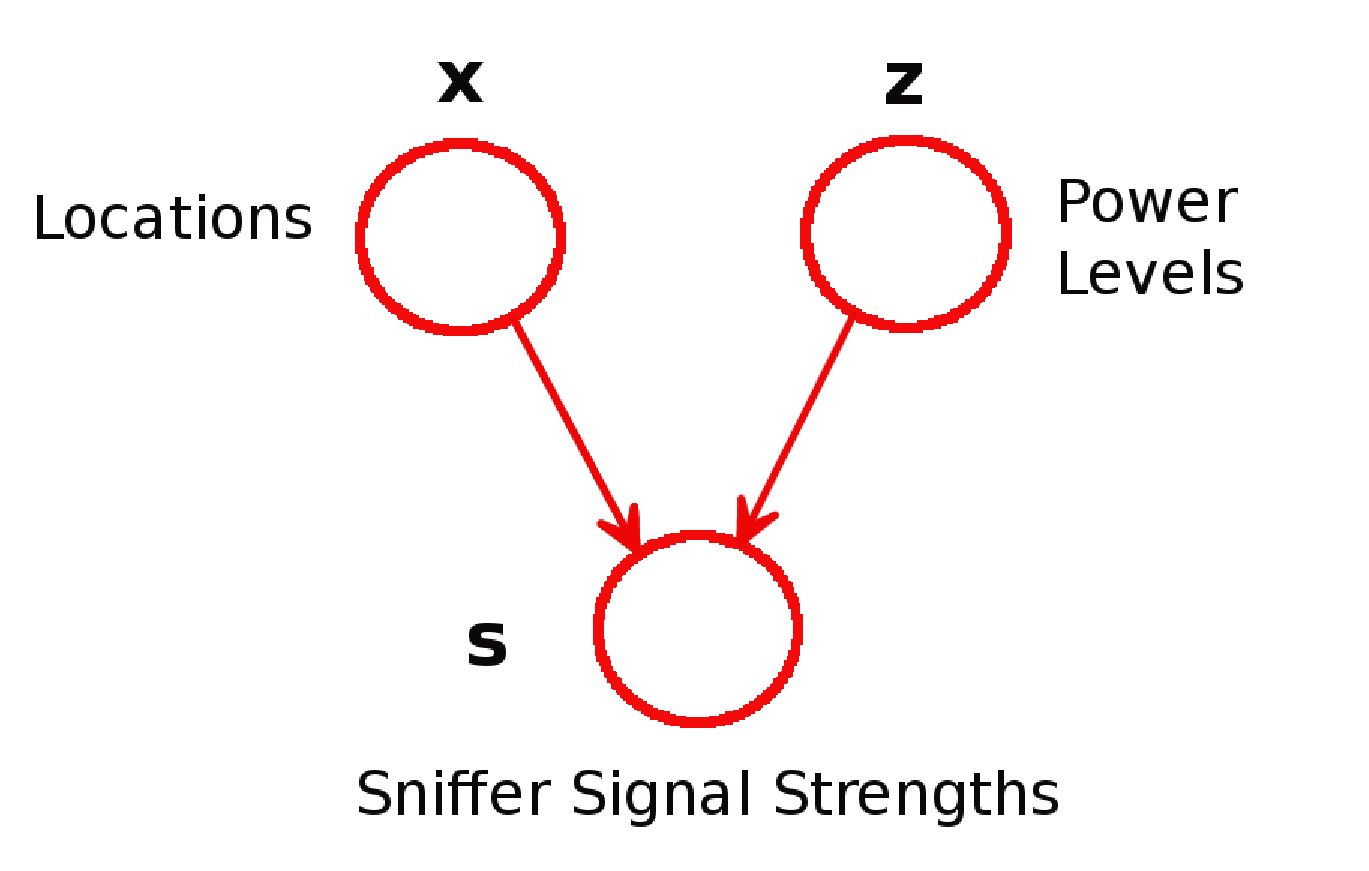
\epsfig{file=Figs4Paper/GMM/gmm4.eps, height=1.2in}
\caption{The GMM for our problem.}
\label{fig:gmm}
\end{figure}


\subsection{RSSI Distribution}
\label{subsec:constructingthedistributionovertheobservedsignalstrengths}

Let $\mathbf{s}$ be the $N$-dimensional vector representing the RSSI observed by the $N$ sniffers in the target area. 
Using the chain rule of probability, we can now define the joint distribution $p(\mathbf{s}, \mathbf{x},\mathbf{z})$ in terms of the distribution $p(\mathbf{x},\mathbf{z})$ and the conditional distribution $p( {\bf s} | {\bf x}, {\bf z})$, 
corresponding to the graphical model in Figure \ref{fig:gmm}:
\begin{align}
p( {\bf s}, {\bf x}, {\bf z}) &= p( {\bf x}, {\bf z}) p( {\bf s} | {\bf x}, {\bf z}).
\end{align}
Since {\bf x} and {\bf z} are independent random variables,
\begin{align}
p( {\bf s}, {\bf x}, {\bf z}) &= p( {\bf x}, {\bf z}) p( {\bf s} | {\bf x}, {\bf z}) \nonumber \\
&= p({\bf x})p({\bf z})p( {\bf s} | {\bf x}, {\bf z}). \label{eqn:joint_distribution}
\end{align}

Equation \ref{eqn:joint_distribution} gives us the joint distribution of $ p( {\bf s}, {\bf x}, {\bf z}) $. The marginal distribution of {\bf s} is then obtained by summing the joint distribution over all possible states of {\bf x} and {\bf z}:
\begin{align}
p( {\bf s}) & = \sum_{\bf x}\sum_{\bf z} p({\bf x})p({\bf z})p({\bf s}|{\bf x}, {\bf z}).\label{eqn:marginal_distribution1}
\end{align}

%\subsubsection{Independence of Sniffers}
%\label{subsubsec:independenceofsniffers}

Now assume that the RSSIs observed at different sniffers are independent. This is justified as the sniffers are typically at disparate locations and thus the wireless propagation path loss can be assumed independent. 
Thus, the term $p( {\bf s} | {\bf x}, {\bf z})$ in equation
\ref{eqn:marginal_distribution1} can be simplified as
\begin{align}
p( {\bf s} | {\bf x}, {\bf z}) & = \prod_{i=1}^N p({s_{i}} | {\bf x}, {\bf
		z}). \label{eqn:conditional_distribution1}
\end{align}
Based on the Gaussian assumption made before, the RSSI can be modeled 
as Gaussian random variables determined by the (location, power-level) pair, so that
\begin{align}
s_{i} | {x_{j}=1}, {z_{k}=1}  \sim  \text{Gaussian}(\mu_{i, (j,k)}, \sigma_{i, (j,k)}).
\end{align}
This lends simplicity to our model since the term $p( {\bf s} | {\bf x}, {\bf z})$ in equation
\ref{eqn:conditional_distribution1} can be expressed succinctly as 
\begin{align}
p( {\bf s} | {\bf x}, {\bf z}) & =  \prod_{j=1}^J \prod_{k=1}^K 
		\prod_{i=1}^N \mathcal{N}(s_{i} |  \mu_{i, (j,k))},\sigma_{i, (j,k)}^2)^{x_j z_k} \, . \label{eqn:conditional_distribution2}
\end{align}
Note that for any given ${\bf x}$ and ${\bf z}$ only one term in the product is actually active for all $i$, because the exponent $x_j z_k$ acts as a selector: $x_j z_k = 1$ for exactly one index pair $(j,k)$, and equals $0$ for all others.

From now on, for notational convenience we define
\[
\mathcal{N}(\mathbf{s} |  \boldsymbol\mu_{(j,k))},\boldsymbol\sigma_{(j,k)}^2) \equiv \prod_{i=1}^N \mathcal{N}(s_{i} |  \mu_{i, (j,k))},\sigma_{i, (j,k)}^2) \, . 
\]

\subsection{Model Parameters}
\label{subsec:modelparameters}

Putting equations \ref{eqn:marginal_distribution1} and
\ref{eqn:conditional_distribution2} together we get the marginal probability distribution over
{\bf s} as
\begin{align}
p( {\bf s}) &= \sum_{j=1}^J \sum_{k=1}^K \upsilon_{j} \tau_{k} \mathcal{N}(\mathbf{s} |  \boldsymbol\mu_{(j,k))},\boldsymbol\sigma_{(j,k)}^2) \, .
\end{align}

Thus we have modeled the marginal distribution of {\bf s} as a Gaussian
mixture with target locations and power levels as the latent variables. The parameters of the model are 
\begin{align}
{\boldsymbol\theta} = \left( {\boldsymbol\upsilon} , {\boldsymbol\tau},  {\boldsymbol\mu} , {\boldsymbol\sigma}^2\right)\, .
\end{align}

Henceforth, we refer to this model as {\bf WiGMM}. We now use the widely popular \emph{Expectation-Maximization} (EM) algorithm~\cite{Dempster77maximumlikelihood, Borman_theexpectation, Bilmes97agentle, DinovIvoD, Bishop:2006:PRM:1162264} to estimate the parameters of the model.

\section{EM Algorithm}
\label{sec:emalgorithm}

An elegant and powerful method for finding maximum likelihood parameter estimates
for probabilistic models with latent variables is the \emph{Expectation Maximization} 
	algorithm. The EM algorithm is an iterative process consisting of two
	steps: an expectation step (E-step) and a maximization step (M-step). During the iterations, a sequence of model parameters ${\bf \theta^{0}}$
, ${\bf \theta^{1}}$, ...., ${\bf \theta^{*}}$ is generated where ${\bf \theta^{0}}$ is the initial parameter and ${\bf \theta^{*}}$ is the converged parameter when the algorithm terminates. Under typical conditions, which hold in our model, the sequence of parameters guarantees monotonic improvement of the likelihood function and almost always converges to a (local) maximum-likelihood estimate.

\subsection{E-step}
\label{subsec:estep}

Suppose we have a data set of RSSI observations at
the sniffers from the target device: ${\bf \overline{S}}$ = \{
${\bf {s}}^{1}$, ${\bf {s}}^{2}$,\ldots,${\bf {s}}^{M}$\}. The E-step
corresponds to finding the expected value of the latent or hidden component ({\bf
		x} and {\bf z}) values given the observed data  ${\bf \overline{S}}$ and the current parameter estimates.
Using this observation set and the current parameter estimates, we find out the posterior probabilities (or responsibilities) as follows. \\

\noindent For each observation ${\bf {s}}^{l}$,
\begin{align}
& \pi_{(j,k)}^{l}  = p({x_{j}} = 1, {z_{k}} = 1 | {\bf{s}}^{l}) \\ 
& = \frac { p({x_{j}} = 1)p({z_{k}} = 1)p( {\bf {s}}^{l} | {x_{j}} = 1, {z_{k}} = 1)} {\ \sum_{p=1}^J \ \sum_{q=1}^{K} p({x_{p}} = 1) p({z_{q}} = 1) p( {\bf {s}}^{l} | {x_{p}} = 1, {z_{q}} = 1)} \nonumber \\ 
& = \frac { \upsilon_{j} \ \tau_{k} \mathcal{N}(\mathbf{s} |  \boldsymbol\mu_{(j,k))},\boldsymbol\sigma_{(j,k)}^2)} {\sum_{p=1}^J \sum_{q=1}^K \upsilon_{p} \tau_{q} \mathcal{N}(\mathbf{s} |  \boldsymbol\mu_{(p,q))},\boldsymbol\sigma_{(p,q)}^2) } \, . 
\end{align}

\noindent The posterior probability value $\pi_{(j,k)}^{l}$ can be viewed as the {\it responsibility} that component $(j,k)$ takes for explaining observation ${\bf {s}}^{l}$. We compute this measure of responsibility for each observation in the data set ${\bf \overline{S}}$.

\subsection{M-step}
\label{subsec:mstep}

The M-step of the algorithm corresponds to maximizing
the \emph{expected} log-likelihood of the observed data. This leads us to re-estimating the parameters for the next iteration based on the posterior probabilities calculated in the expectation step of the algorithm
\begin{align}
\upsilon_{j} = \frac { \sum_{l=1}^{M} \ \sum_{k} \pi_{(j,k)}^{l}} {M},
\end{align}
\begin{align}
\tau_{k} = \frac { \sum_{l=1}^{M} \ \sum_{j} \pi_{(j,k)}^{l}} {M},
\end{align}
\begin{align}
\mu_{i \ (j,k)} = \frac  { \sum_{l=1}^{M} \pi_{(j,k)}^{l} s_{i}^{l}} {N_{j,k}},
\end{align}
where
\begin{align}
{N_{j,k}} = \sum_{l=1}^{M} \pi_{(j,k)}^{l}.
\end{align}

The variance parameter can also be updated accordingly.

\subsection{Convergence of Log Likelihood}
\label{subsec:convergenceofloglikelihood}

\begin{figure}
\centering
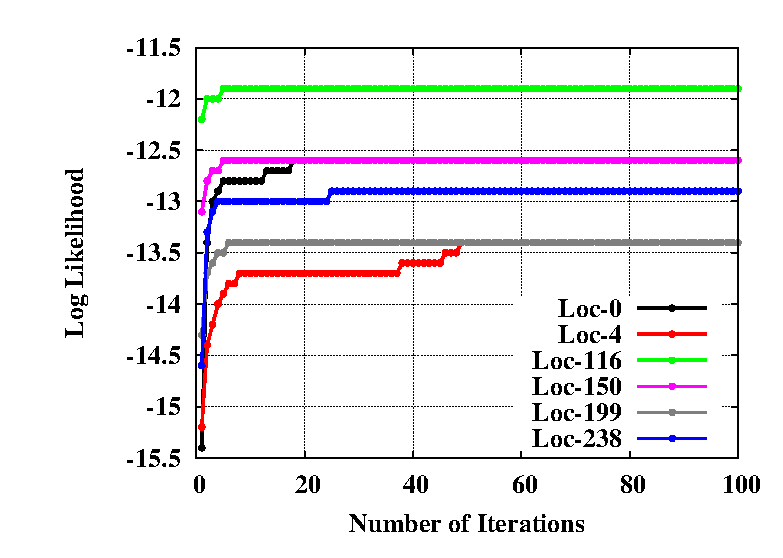
\epsfig{file=Figs4Paper/CEWIT/GMM-LogLikelihood/LogLikelihood.eps, height=1.5in, width=2.5in}
\caption{Convergence of log likelihood for 6 different instances of using WiGEM.}
\label{fig:loglikelihood}
\end{figure}

Each update of the parameters resulting from an E-step followed by an
M-step is guaranteed to increase the log likelihood function
\begin{align}
\ln p({\bf \overline{S}} | {\bf \theta}) &= \sum_{l=1}^{M} \ln \left\{
\sum_{j=1}^J \sum_{k=1}^K \upsilon_{j} \tau_{k} \mathcal{N}(\mathbf{s} |  \boldsymbol\mu_{(j,k))},\boldsymbol\sigma_{(j,k)}^2) \right\}.
\end{align}

The algorithm is deemed to have converged when the change in the log likelihood function between two successive iterations falls below a threshold ($10^{-6}$ in the experiments described later). 
Figure~\ref{fig:loglikelihood} shows how the log-likelihood converges for six different instances of running WiGEM. Each instance here is to localize an Android phone on the CEWIT testbed (Section \ref{subsec:testbeddetails}). \\ 

%Hereafter, we refer to our algorithm as {\bf WiGEM}.

\subsection{Handling Identifiability in WiGEM}
\label{subsec:handlingidentifiabilityinourmodel}

There is an identifiability problem in this general approach that is well understood~\cite{Bishop:2006:PRM:1162264}. This arises because there are $U!$ equivalent solutions
in a $U$ component mixture model. In our case,
each component is a (location,
power-level) pair. 
We handle the problem of identifiability 
by using the knowledge of sniffer locations to initialize the EM algorithm
using the basic log-distance radio propagation model~\cite{Rappaport:2001:WCP:559977, Molkdar91} below :
%\subsubsection{Indoor Radio Propagation Model}
%\label{subsubsec:indoorradiopropagationmodel}
\begin{align}
P_r(d) = G\frac{P_t}{d^\alpha},
\end{align}
where $P_r(d)$ is the received power at distance $d$ and $P_t$ is the transmit power.
$\alpha$ is the path loss exponent which is simply a model parameter. 
In free space $\alpha =2$, but it typically increases somewhat in complex 
environments. $G$ is a frequency and antenna dependent constant. 
Often the above equation is expressed somewhat differently as 
\begin{align}
P_r(d) = P_r({d_0}) - 10\alpha\log\left(\frac {\it d} {\it d_{0}}\right)
	\label{eqn:pathloss_1},
\end{align}
%\noindent
where $P_r$ is now expressed in decibel (dB) units. This emphasizes that when powers 
are expressed in dB units transmit power changes expressed in dB cause the same dB change at all receivers
regardless of location. In our experiments we will use RSSI in dB units. We independently
verified (not reported here for brevity) that the RSS measurement on our sniffer hardware is accurate at least to the extent
that a dB shift in the transmit power does get recorded as a similar
shift at the sniffer regardless of location.

%\subsubsection{Reference Signal Power and the Path Loss Parameter}
%\label{subsubsec:referencesignalpathloss}
%
%In Equation \ref{eqn:pathloss_1},  $P_r({d_0})$ is the signal power at
%some reference distance $d_{0}$ from the sniffer. This reference signal
%strength $P_r({d_0})$ can be derived empirically or obtained from
%wireless network hardware specifications \cite{Bahl00radar:an}. In our
%deployment all our sniffers have the same hardware (described in detail
%		in Section \ref {sec:evaluation}) . The value of $P_r({d_0})$
%was empirically found to be approximately 60 dB when $d_{0}$ = 1 meter . No assumption is made about the
%target space, so $\alpha =2$. The path loss equation of equation
%\ref{eqn:pathloss_1} can now be succintly expressed as 
%\begin{align}
%P_r(d) = 60 - 10\alpha\log\left({\it d} \right)  .
%	\label{eqn:pathloss_2}
%\end{align}

\subsubsection{Initializing the Model Parameters}
\label{subsubsec:initializingthecomponentsofourmodel}

\begin{itemize}

\item ${\boldsymbol\upsilon}$ and ${\boldsymbol\tau}$ are initialized as being from a uniform distribution over locations and power levels respectively.

\item For a location $l_{j}$, Equation \ref{eqn:pathloss_1} gives us the theoretical RSSI value  $w_{ij}$ (say) at a sniffer $s_{i}$. The reference power $P_r({d_0})$
is assumed to be 60 (in dB units) at $d_0=1$ meter. Note that the reference power
assumption is somewhat arbitrary. The parameter $\alpha$ is assumed to be 2. 

We consider $K$ values reflecting the power levels:
\begin{align}
\left\{ (w_{ij}-\frac{K}{2}), (w_{ij}-\frac{K}{2}+1), \dots ,(w_{ij}+\frac{K}{2})\right\}. \nonumber
\end{align}
The values are used to initialize the means, $\mu_{i, (j,k)}$ of the $K$ components corresponding to location $l_{j}$ and sniffer $s_{i}$. We do this for every target location in the map and for each sniffer in the building. This effectively initializes parameter ${\boldsymbol\mu}$ in WiGMM. 

Note: negative values are not allowed and are set to 0 during initialization.

\item The standard deviation parameter, ${\boldsymbol\sigma}$, is initialized to 5 for each component in WiGMM (and kept fixed to reduce computation time). This choice is mostly arbitrary. Some previous work \cite{Tao:2003:WLL:941311.941314} also use fixed values of standard deviation ($\sigma=12$) in their work. \\

\end{itemize}

%, that should be observed at the
%sniffer for a client transmitting from $l_{i}$. 

% However, different devices may work at different power-levels
% for doing wireless transmissions. To handle this scenario, we consider $K$ values for each location $l_{i}$:
% \begin{align}
% \{ (w_{i}-\frac{K}{2}), (w_{i}-\frac{K}{2}+1), \dots ,(w_{i}+\frac{K}{2})\}.
% \end{align}
% Use these values to initialize the means for the $K$ different
% components corresponding to location $l_{i}$. Recall from Section \ref{subsec:latentvariablesfortargetlocationsandpowerlevels}, that WiGMM has a $K$-dimensional binary random variable $\mathbf{z}$ representing Power Levels.     {\bf We do this procedure for every possible
% target location in the map, so that we initialize the mean of every component in WiGMM}.  The standard deviation ($\sigma_{j, k}$)
% 	was chosen as 5 (and kept fixed to reduce computation time). This
% 	choice was mostly arbitrary though some previous work
% 	\cite{Tao:2003:WLL:941311.941314} also use fixed values of standard
% 	deviation ($\sigma=12$) in
% 	their work. 

\subsection{Final Location Estimate}
\label{subsec:finallocationestimate}

\begin{figure}
	\centering
		\subfloat[CEWIT]{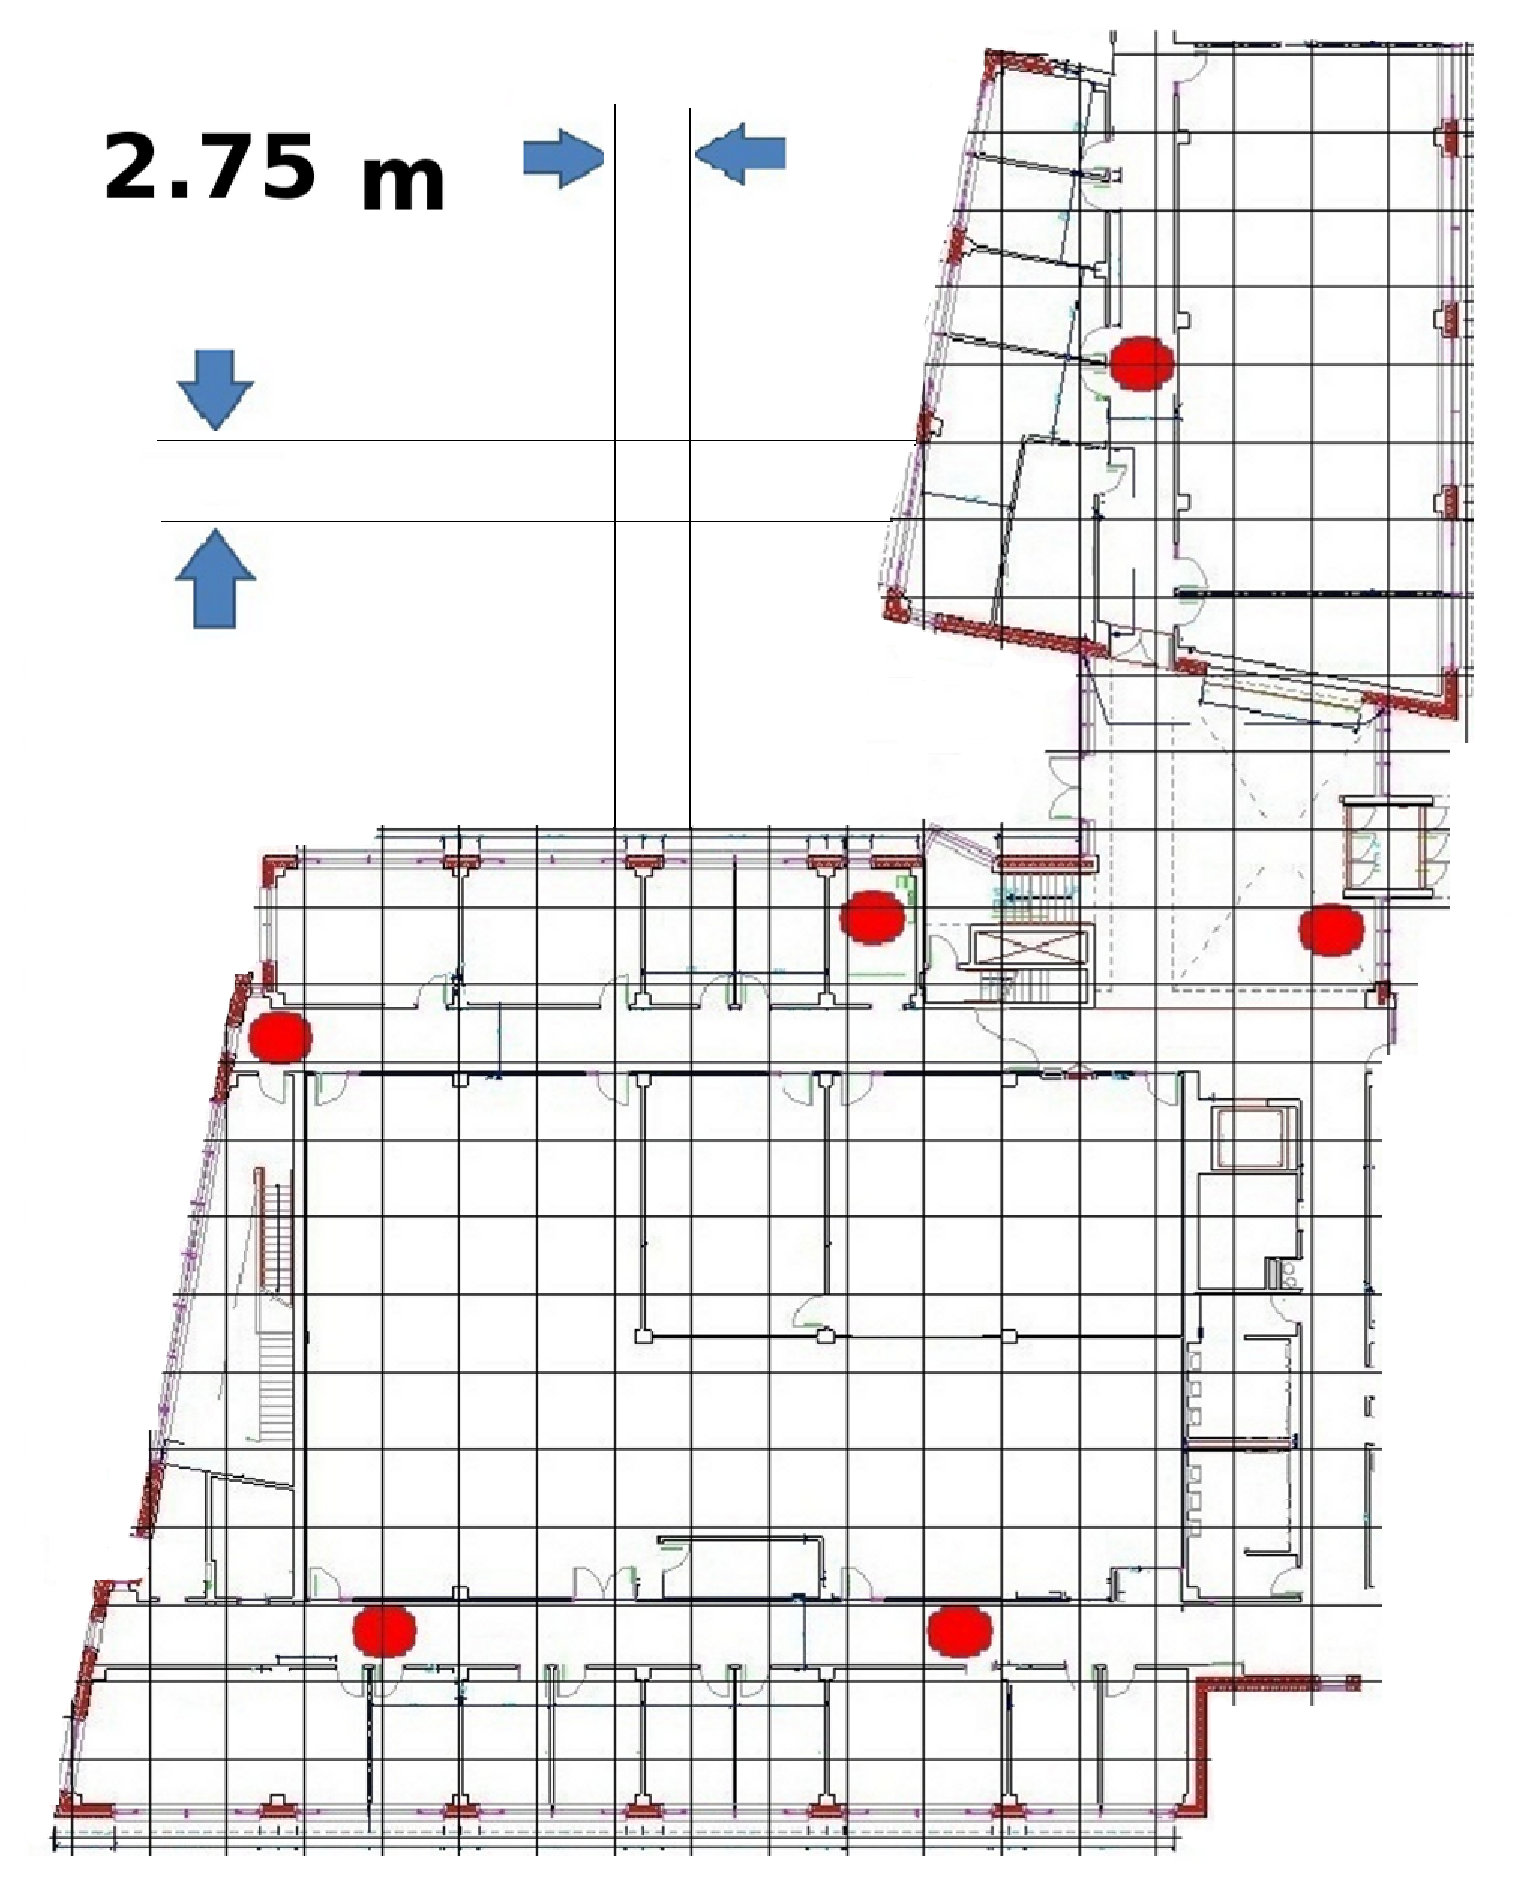
\includegraphics[height=1.8in]{Figs4Paper/CEWIT/CEWIT-Map7.eps}} \quad \quad \\
		\subfloat[CSD]{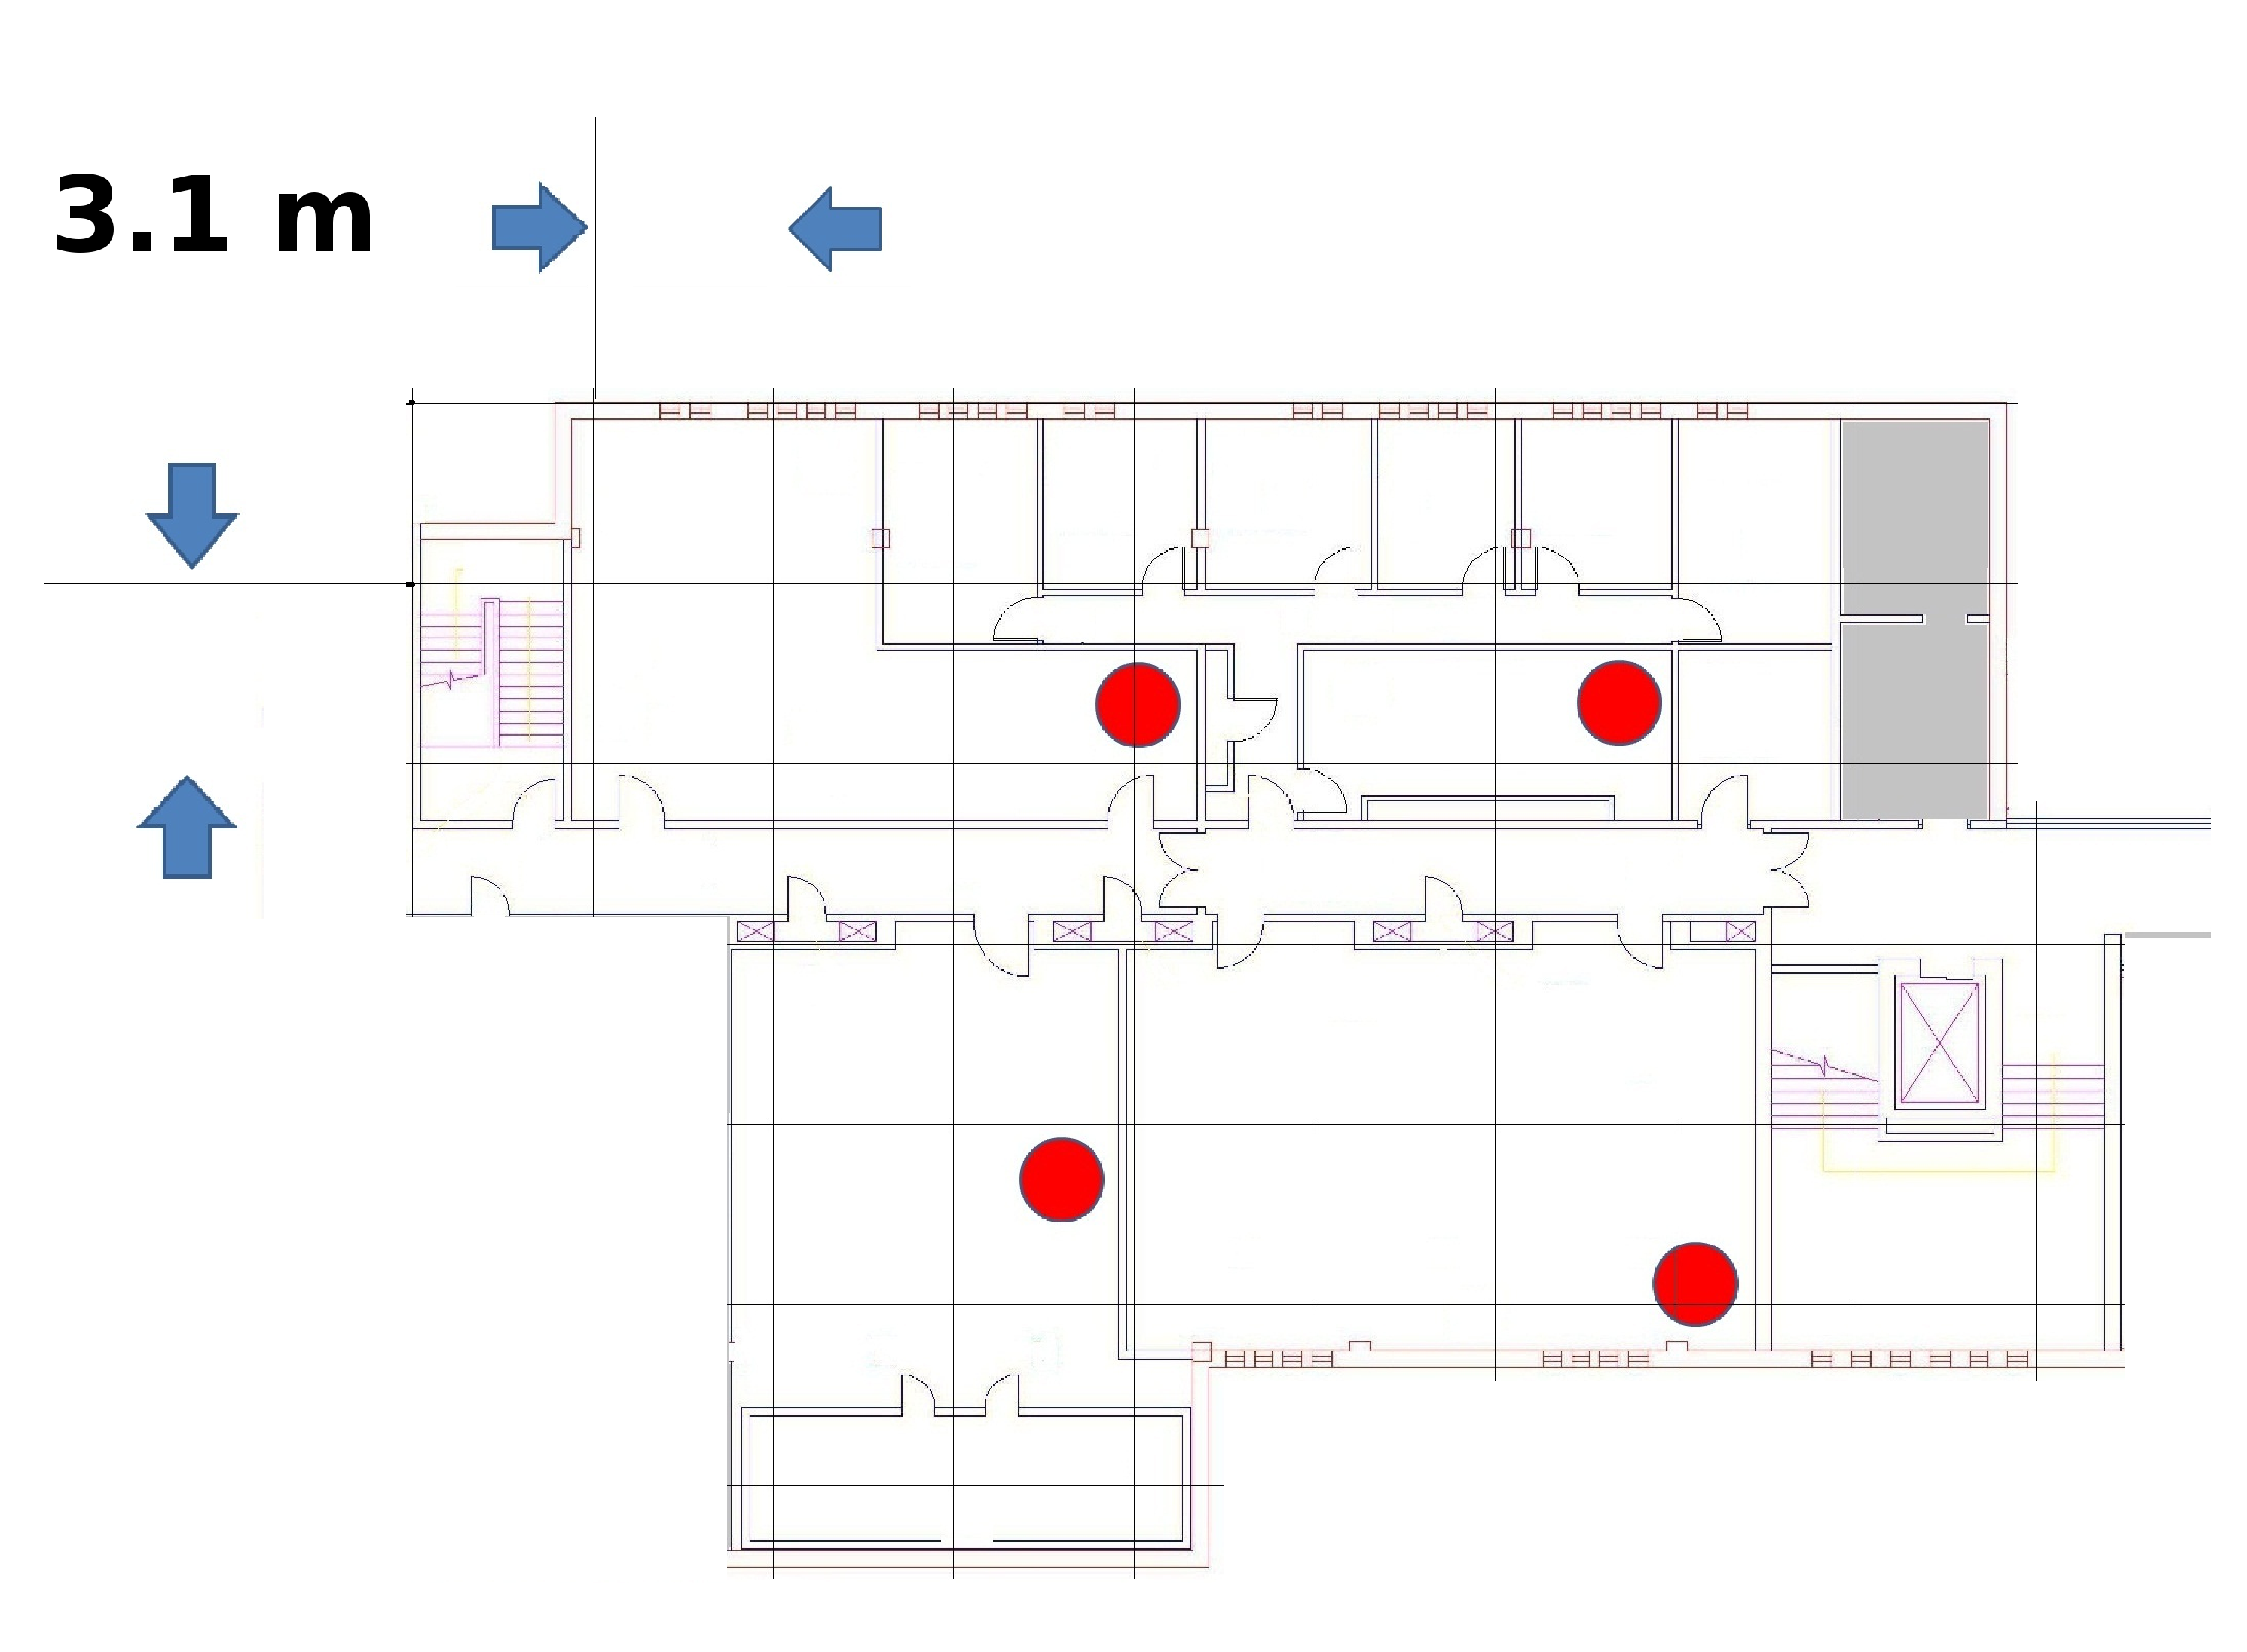
\includegraphics[width=2in]{Figs4Paper/CSD/CSD-Map4.eps}} 
	\caption{Two testbeds for validation experiments. The finer grids are 
	shown (see text). The red circles represent sniffer locations.}
	\label{fig:experimenttestbed}
\end{figure}


Given a real-time received RSSI vector ${\bf {s}}^{(obs)}$, we can now
find the location with the highest probability. We do this by first
finding the probability for each (location, power-level) pair and then
marginalizing over the power-levels. This gives us a probability
distribution over the possible locations inside the target space. The
location with the highest probability is returned as the answer.
Thus the estimated location index is given by $j^{*}$, where
\begin{align}
j^{*} = \arg\max_{j} \sum_{k} p({x_{j}} = 1, {z_{k}} = 1 | {\bf {s}}^{(obs)}) \, .
\end{align}

\section{Experiment Methodology}
\label{sec:experimentmethodology}

We start with a description of our system setup, including an overview of the components of our sniffer devices. We then present details about the two testbeds where we conducted our experiments. Finally, we round up this section by discussing the data collection process.

\subsection{System Setup}
\label{subsec:systemsetup}

As mentioned briefly in Section \ref{sec:introduction}, WiGEM uses an infrastructure based
architecture. The system has two main components: stationary sniffer devices in the target space and a centralized server running the WiGEM algorithm. Sniffers provide overlapping coverage of the target area (similar to WLAN APs). The server notifies the sniffers about the MAC id of the target device, the channel number and the listening period. The sniffers then record the RSSI of all packets received that match the server's query. The recorded information is sent to the server which then makes a location estimation using the WiGEM algorithm.

In the current prototype, the server communicates with the sniffer devices using in-building power-line network. In the ultimate embodiment, the sniffer functionality could be integrated directly into the WLAN APs. If necessary and appropriate, a localization application can also run on the client that downloads the building map as soon as it gets connected to the WLAN, sends a localization request to the WLAN and shows the location on the map. 

\subsubsection{Sniffer Information}
\label{subsec:snifferinformation}

%The sniffer devices are responsible for capturing wireless transmissions made by a Tx-client. 

We use Soekris net4801~\cite{soekris}  SBCs as sniffer
devices with atheros-based CM9 cards for wireless captures. The sniffers run Pyramid Linux (version 2.6.16-metrix). The default
MadWiFi driver is used which comes with this distribution (0.9.4.5:svn 1485). 

To capture packets the standard Tcpdump tool (version 4.0.0/libpcap version 0.9.8) is used. To obtain signal strength information, the MadWiFi driver allows a
monitor mode interface to be created and configured with the radio tap header support. 
The radio tap header reports the SNR (in dB) as the RSSI. This is what we use directly. 
Since the noise floor reported by the cards is constant (-95dBm), the RSSI value 
is also the same as the RSS (in dBm) with a constant difference. 

%ra header we can extract the
%RSSI of each packet received by the sniffer. We verified that the MadWifi driver had a fixed noise-floor in each of our
%cm9 cards (-95 dbm). In fact the received signal strength of a frame reported by the MadWiFi driver is actually the SNR value (in db) obtained after subtracting the noise-floor from the raw signal strength value. We work directly with the RSSI value (in db) as reported by the driver.

\subsection{Testbed Details}
\label{subsec:testbeddetails}

Two different indoor testbeds are used for validation. The first building, henceforth called CEWIT, is a research and development center at Stony Brook University with a dimension of 65 meter $\times$ 50  meter. The L-shaped floor comprises of several obstructions in the form of walls of various types, glass and metal doors, office furnitures, server-rack cabinets etc. The second building, henceforth called CSD, is part of the building housing the Computer Science Department at Stony Brook University. This rectangular-shaped floor has a dimension of 20 meter $\times$ 30 meter, and also has walls, various partitions and office furnitures. Both these testbeds had a continuous flux of people moving around in the building at the time
the experiments were conducted. The CEWIT and CSD testbeds use 6 and 4 sniffers respectively. 
See Figure~\ref{fig:experimenttestbed} for the sniffer locations. 

\subsection{Data Collection Methodology}
\label{subsec:datacollectionmethodology}

%{\color{red} The CEWIT testbed has 45 distinct test locations roughly every 5.5 meters. The CSD testbed has 27 distinct test locations roughly every 3.3 meters. The testing locations are uniformly distributed in each testbed. Note that test locations are a subset of the total number of vertices formed by a superimposed (virtual) grid. The grid vertices are 2.75 meters apart for the CEWIT testbed and 3.1 meters apart for the CSD testbed (Figure~\ref{fig:experimenttestbed}).} 

We discretize the physical space in each testbed individually using 
a superimposed virtual grid (Figure~\ref{fig:experimenttestbed}). A side of the grid square
is 2.75m for the CEWIT testbed and 3.1m for the CSD testbed. The grid vertices serve as the possible
target locations for WiGMM. Let us refer to this grid as the `finer' grid.  The granularity of this grid impacts
computation time and accuracy of WiGEM, with finer granularity likely to work better. However, there is no 
labor cost for data collection with finer granularity. 

Another slightly `coarser' grid  (5.5m side for CEWIT and 3.3m side for CSD) is used where the vertices
serve as
the `test' locations. The CEWIT testbed has 45 distinct test locations  and the CSD testbed has 27 distinct test locations. The test locations are thus uniformly distributed in each testbed.  Multiple device types are used. For each device, we transmit 200 ping packets from every distinct test location of the corresponding testbed. This is typically accomplished by having 
the user hold the mobile device and walk across the floor of the building briefly stopping at each marked test location to transmit 200 ping packets. The ground truth is noted at each location before moving on to the new location. Note that the ground truth information is used only for evaluation of the localization error and is not supplied to WiGEM for training. Each ping packet is separated uniformly apart at a rate of 1 per second. On the server, the sequence number in the ping packet is used to form the vector of RSSI values recorded by individual sniffers for each transmission. Thus, from each distinct test location on the map and for each device type, we have a set of 200 RSSI tuples. This comprises our entire data set that we use in this paper. 

\subsubsection{Test Devices}
\label{subsubsec:testdevices}

Four different wireless devices are used - a Laptop, an Android phone, an iPhone and a Netbook. The laptop is a Dell Inspiron 1545 running Ubuntu v9.04. The Android phone is a Google Nexus One. The iPhone is iPhone 3GS (iOS version 4.2.1). The netbook is a Dell Latitude 2110 running Ubuntu v9.10. Each device uses its default driver and default power levels for WiFi transmissions. %The devices are henceforth referred to as {\it Laptop}, {\it Android}, {\it iPhone} and {\it Netbook} respectively. 
No special setup or changes are done on the devices related to networking or WiFi interfaces. 
Thus, the devices use their default rate and power control, if any.
The data is collected over a span of several days. The devices are not oriented
in any specific direction while making the ping transmissions. The orientation is simply left to the user's choice or convenience. 

%\subsubsection{Sniffer Position}
%\label{subsubsec:snifferposition}
%
%The CEWIT and CSD testbeds have six and four sniffers respectively. See Figure \ref{fig:experimenttestbed}. We assume knowledge of the sniffer positions in the map and use this information to calculate the signal strength values given by the indoor radio propagation model (Equation \ref{eqn:pathloss_2}). These values are used to initialize our algorithm as explained in Section \ref{subsec:handlingidentifiabilityinourmodel} .

\section{Evaluation}
\label{sec:evaluation}

In this section, we present the evaluation of WiGEM on the two different testbeds. 
Our test cases include heterogeneous devices as described before with unmodeled hardware and power level characteristics, this providing a very realistic
benchmarking. We also compare WiGEM with respect 
to a simple propagation model based scheme (that also requires no pre-deployment effort) as well as well-known, high-performing schemes such as RADAR and Probabilistic~\cite{Haeberlen:2004:PRL:1023720.1023728,Youssef:2008:HLD:1399551.1399558,Roos} (they require significant pre-deployment effort, but provide the best accuracy). In addition we evaluate how the size
of the learning data set or mobility impacts the accuracy of WiGEM. 

%we present a comprehensive overview of our experimental results. We evaluate the performance of WiGEM on our two experimental testbeds. We attempt to answer the following questions.
%
%\begin{itemize}
%
%\item What is the number of power-levels that we should use in WiGMM i.e what is the value of K (mentioned in Section \ref{subsec:latentvariablesfortargetlocationsandpowerlevels} above) that we should use when we run WiGEM on the back end localization server ? 
%\item How does the WiGEM localization accuracy vary as the size of the learning data-set increases ?
%\item What is the WiGEM accuracy for heterogenous devices with unmodelled hardware and power-level characteristics ?
%\item How does WiGEM perform with respect to a model-based scheme that uses the indoor radio path loss propagation model ? This presents a true head-to-head comparison because neither needs pre-deployment effort and can work on the same granularity of discretization of the target space.
%\item How does WiGEM perform with respect to schemes that build RF signal maps like RADAR and Probabilistic \cite{Haeberlen:2004:PRL:1023720.1023728, Youssef:2008:HLD:1399551.1399558, Roos} . This experiment shows how the WiFi hardware variance problem can impact the accuracy of RF signal map schemes and also show the impact of training granularity for signal map based schemes.
%\item Can the mobility of a client can actually improve WiGEM's localization accuracy ?
%
%\end{itemize}


All reported experiments with WiGEM uses half of the measured data set at each test location for learning and the other half for testing and validation. The learning part reflects the typical learning process for WiGEM.
The general idea is that a typical client device will naturally transmit multiple (likely many) packets for its own network use. It can always be forced to transmit some number of packets for use in localization if it does not naturally transmit anything. The sniffed RSSI vectors for these packets will form the learning set to be used in WiGEM localization. The client does not need to be stationary and is free to move about while the learning set is gathered. In practice, we could keep doing the EM steps and generating location estimates as the device moves through the environment.  Unless otherwise noted, we conduct our experiments across all test locations (Section \ref{subsec:datacollectionmethodology}). Likewise, the error distances reflect the aggregate metric across all test locations.  Two important questions now are the determination of a suitable number of power levels ($K$) to use for the learning and the size of learning set. These are addressed next.

%As mentioned in Section \ref{subsec:datacollectionmethodology} above, the CEWIT testbed has 45 distinct locations and CSD has 27 distinct locations, and for each distinct location on the map and for each device type we have a set of 200 RSS tuples. 
%We divide these 200 tuples into two sets of 100 tuples each: one for learning the WiGMM parameters and the other for testing the WiGEM localization results. Each device type is considered separately. 
%

\subsection{Number of Powers Levels and Learning Set Size}
\label{subsec:numberofpowerlevelstouseingem}

\begin{figure}[h!]
	\centering
		\subfloat[{\small CEWIT testbed}]{\includegraphics[height=1.25in, width=1.6in]{Figs4Paper/CEWIT/PowerPlot4Paper_CEWIT/PwrLvlPlot_cewit.eps}} 
		\subfloat[{\small CSD testbed}]{\includegraphics[height=1.25in, width=1.6in]{Figs4Paper/CSD/PowerPlot4Paper_CSD/PwrLvlPlot_csd.eps}}
	\caption{Average error distance results for WiGEM
	as a function of the number of power levels.}
	\label{fig:powerlevelsvserrordistance}
\end{figure}

%\begin{figure*}
%	\centering
%		\subfloat[CEWIT testbed]{\includegraphics[height=1.5in, width=2.5in]{Figs4Paper/CEWIT/PowerPlot4Paper_CEWIT/PwrLvlPlot_cewit.eps}}
%		\subfloat[CSD testbed]{\includegraphics[height=1.5in, width=2.5in]{Figs4Paper/CSD/PowerPlot4Paper_CSD/PwrLvlPlot_csd.eps}}
%	\caption{Average error distance results for WiGEM
%	as a function of the number of power levels.}
%	\label{fig:powerlevelsvserrordistance}
%\end{figure*}


As a part of the evaluation, we determine the number of power levels ($K$) that should 
be used for the modeling. Note again that the use of power levels is simply a modeling convenience; the 
actual transmit power of the device is not influenced in any fashion. Figure \ref{fig:powerlevelsvserrordistance} shows the results of the average error distance (in meters) for the four devices across  varying number of power levels used in WiGEM. We see that the average error distance hits a plateau after $K = 31$. This is an interesting result because it helps us bound the number of power levels to use. We use a value of $K = 45$ in the subsequent experiments. 

%\subsection{Localization accuracy in WiGEM as a function of the learning set size.}
%\label{subsec:localizationaccuracyasafunctionofthelearningsetsizeingem}
%
\begin{figure}[h!]
\centering
		\subfloat[{\small CEWIT testbed}]{\includegraphics[height=1.25in, width=1.6in]{Figs4Paper/CEWIT/LearningSize4Paper_CEWIT/LearningSetSize_cewit.eps}}
		\subfloat[{\small CSD testbed}]{\includegraphics[height=1.25in, width=1.6in]{Figs4Paper/CSD/LearningSize4Paper_CSD/LearningSetSize_csd.eps}}
  %\epsfig{file=Figs4Paper/CEWIT/LearningSize4Paper_CEWIT/LearningSetSize_cewit.eps, height=1.5in, width=2.5in}
  \caption{Average error distance results for WiGEM
   as a function of the learning set size.}
  \label{fig:learningsetsizevserrordistance}
\end{figure}

Having fixed the number of power levels to use, we now study how the size of the learning data set changes the average error distance. Recall here that as part of our data collection methodology, we have 200 RSS tuples for every location on the map for each of the four device types. This time we again divide the 200 tuples into two sets: one set for learning and the other for testing. The test set size is kept fixed at 100 RSS tuples. From the remaining tuples, the learning set size is varied from 2 tuples going up to 100 tuples. Figure~\ref{fig:learningsetsizevserrordistance} shows the results of the average error distance (in meters) as the size of the learning set varies. For the CEWIT testbed, we observe that for all the four devices, the average error does not vary much as we move from 50 training samples to 100 training samples. The CSD testbed results converged after 10 samples itself. The experiments that follow have been done keeping the WiGEM learning set size at 100 and using the remaining 100 samples for testing the localization accuracy.  Experiments on RADAR and Probabilistic (described later in this paper) use the corresponding datasets for building the RF signal map and calculating localization error respectively.


\subsection{WiGEM Accuracy With Heterogeneous Devices}
\label{subsec:gemaccuracyforheterogeneousdevices}

\begin{figure}
	\centering
	\begin{tabular}{cc}
	\subfloat[{\small CEWIT testbed}]{\includegraphics[height=1.25in, width=1.6in]{Figs4Paper/CEWIT/Gem4Devices_CEWIT/4Devices_cewit.eps}} &
	      \subfloat[{\small CSD testbed}]{\includegraphics[height=1.25in, width=1.6in]{Figs4Paper/CSD/Gem4Devices_CSD/4Devices_csd.eps}}
	\end{tabular}      
	\caption{CDF of WiGEM's location accuracy for multiple devices.}
	\label{fig:gemheterogeneousdevices}
\end{figure}

%\begin{figure*}
%	\centering
%	      \subfloat[CEWIT testbed]{\includegraphics[height=1.5in, width=2.5in]{Figs4Paper/CEWIT/Gem4Devices_CEWIT/4Devices_cewit.eps}}
%	      \subfloat[CSD testbed]{\includegraphics[height=1.5in, width=2.5in]{Figs4Paper/CSD/Gem4Devices_CSD/4Devices_csd.eps}}
%	\caption{CDF of WiGEM's location accuracy for multiple devices.}
%	\label{fig:gemheterogeneousdevices}
%\end{figure*}

Figure \ref{fig:gemheterogeneousdevices} plots CDFs of error distances showing how WiGEM performs across the four test devices. % (Section \ref{subsubsec:testdevices}). 
For both the testbeds, the accuracy estimates are pretty similar for all the devices. Thus, we see that WiGEM can adapt itself for heterogeneous devices that possibly work at different transmit power levels. In Section \ref{subsec:comparisonswithschemesthatuserfsignalmaps}, we show how RF-signal map based techniques show substantial degradation in accuracy owing to such hardware variations. 

\subsection{Baseline Comparison with a Model-based Scheme}
\label{subsec:baselinecomparisonwithamodelbasedscheme}

\begin{figure}[h!]
	\centering
	      \subfloat[{\small CEWIT testbed}]{\includegraphics[height=1.25in, width=1.6in]{Figs4Paper/CEWIT/Baseline4Paper_CEWIT/BaselineComparisonsMedianError_cewit.eps}}
	      \subfloat[{\small CSD testbed}]{\includegraphics[height=1.25in, width=1.6in]
	      {Figs4Paper/CSD/Baseline4Paper_CSD/BaselineComparisonsMedianError_csd.eps}}
	\caption{Baseline Comparisons.}
	\label{fig:baselinecomparisons}
\end{figure}

%\begin{figure*}
%	\centering
%	      \subfloat[CEWIT testbed]{\includegraphics[height=1.5in, width=2.5in]{Figs4Paper/CEWIT/Baseline4Paper_CEWIT/BaselineComparisonsMedianError_cewit.eps}}
%	      \subfloat[CSD testbed]{\includegraphics[height=1.5in, width=2.5in]
%	      {Figs4Paper/CSD/Baseline4Paper_CSD/BaselineComparisonsMedianError_csd.eps}}
%	\caption{Baseline Comparisons.}
%	\label{fig:baselinecomparisons}
%\end{figure*}

%% \begin{figure*}
%% \begin{minipage}{0.5\textwidth}
%% 	{\centering
%% 	  \subfloat[Probabilistic]{\includegraphics[width=0.5\textwidth]{Figs4Paper/CEWIT/HRComparisons4Paper_CEWIT/HRComparisonsMedianError_Probabilistic_cewit.eps}}
%% 	  \subfloat[RADAR]{\includegraphics[width=0.5\textwidth]{Figs4Paper/CEWIT/HRComparisons4Paper_CEWIT/HRComparisonsMedianError_RADAR_cewit.eps}}
%% 	\caption{Comparisons on the CEWIT Testbed}
%% 	\label{fig:HR_on_cewittestbed}
%% 	}
%% \end{minipage}\quad
%% \begin{minipage}{0.5\textwidth}
%% 	{\centering
%% 		\subfloat[Probabilistic]{\includegraphics[width=0.5\textwidth]{Figs4Paper/CSD/HRComparisons4Paper_CSD/HRComparisonsMedianError_Probabilistic_csd.eps}}
%% 		\subfloat[RADAR]{\includegraphics[width=0.5\textwidth]{Figs4Paper/CSD/HRComparisons4Paper_CSD/HRComparisonsMedianError_RADAR_csd.eps}}
%% 	\caption{Comparisons on the CSD Testbed}
%% 	\label{fig:HR_on_csdtestbed}
%% 	}
%% \end{minipage}
%% \end{figure*}

Now we analyze the performance of WiGEM with respect to a model-based scheme that uses the indoor radio propagation model (Section~\ref{subsec:handlingidentifiabilityinourmodel}). 
Neither of the techniques need pre-deployment effort. We want to basically establish that
the learning technique used in WiGEM is buying us something relative to a generic radio
propagation model. 
% Both our testbeds, CEWIT and CSD, have been discretized as shown in Figure \ref{fig:experimenttestbed}. There are 267 grid vertices inside the CEWIT testbed roughly every 2.75 meters. The CSD testbed has 36 grid vertices roughly every 3.1 meters. WiGEM can localize a given target RSS vector to any of these grid vertices. As mentioned in Section \ref{subsec:datacollectionmethodology}, the data for our experimental evaluation is coming from 45 distinct locations on the CEWIT testbed and 27 distinct locations in the CSD testbed. There are 200 RSS tuples for every location on the map for each of the four device types. As mentioned above in Section \ref{subsec:localizationaccuracyasafunctionofthelearningsetsizeingem}, WiGEM is using a learning set size of 100 RSS samples with 45 power levels to build the WiGMM model. Thus the test-set for both the algorithms is remaining 100 RSS tuples from each location. Each device type is evaluated separately.

The log-distance path loss mentioned in Section~\ref{subsec:handlingidentifiabilityinourmodel} is used to estimate the RSS that should be observed at a sniffer for each grid vertex (for the finer grid) inside the target space. These RSS values are used to initialize WiGEM, as mentioned in Section~\ref{subsec:handlingidentifiabilityinourmodel}. The model-based algorithm also uses these same RSS values with a suitable metric to give a final location estimate. Similar to \cite{Bahl00radar:an}, the model-based algorithm that we use here uses the `nearest neighbor in signal space' as the metric of choice. 
Figure~\ref{fig:baselinecomparisons} shows the median error for both techniques. Note that WiGEM performs better than the model-based scheme across all device types in both testbeds. The performance improvement is quite substantial for the phone-based devices -- with the median error distance reducing to roughly half. 

\subsection{Comparison with Schemes Using RF Signal Maps}
\label{subsec:comparisonswithschemesthatuserfsignalmaps}

\begin{figure}[h!] 
	\centering
	      \subfloat[{\small WiGEM vs. Probabilistic}]{\includegraphics[height=1.25in, width=1.6in]{Figs4Paper/CEWIT/HRComparisons4Paper_CEWIT/HRComparisonsMedianError_Probabilistic_cewit.eps}}
	      \subfloat[{\small WiGEM vs. RADAR}]{\includegraphics[height=1.25in, width=1.6in]
	      {Figs4Paper/CEWIT/HRComparisons4Paper_CEWIT/HRComparisonsMedianError_RADAR_cewit.eps}}
	\caption{Comparisons on the CEWIT testbed.}
	\label{fig:HR_on_cewittestbed}
\end{figure}

\begin{figure}[h!]
	\centering
	      \subfloat[{\small WiGEM vs. Probabilistic}]{\includegraphics[height=1.25in, width=1.6in]{Figs4Paper/CSD/HRComparisons4Paper_CSD/HRComparisonsMedianError_Probabilistic_csd.eps}}
	      \subfloat[{\small WiGEM vs. RADAR}]{\includegraphics[height=1.25in, width=1.6in]
	      {Figs4Paper/CSD/HRComparisons4Paper_CSD/HRComparisonsMedianError_RADAR_csd.eps}}
	\caption{Comparisons on the CSD testbed.}
	\label{fig:HR_on_csdtestbed}
\end{figure}

%\begin{figure*}
%	\centering
%	      \subfloat[WiGEM vs. Probabilistic]{\includegraphics[height=1.5in, width=2.5in]{Figs4Paper/CEWIT/HRComparisons4Paper_CEWIT/HRComparisonsMedianError_Probabilistic_cewit.eps}}
%	      \subfloat[WiGEM vs. RADAR]{\includegraphics[height=1.5in, width=2.5in]
%	      {Figs4Paper/CEWIT/HRComparisons4Paper_CEWIT/HRComparisonsMedianError_RADAR_cewit.eps}}
%	\caption{Comparisons on the CEWIT testbed.}
%	\label{fig:HR_on_cewittestbed}
%\end{figure*}
%
%\begin{figure*}
%	\centering
%	      \subfloat[WiGEM vs. Probabilistic]{\includegraphics[height=1.5in, width=2.5in]{Figs4Paper/CSD/HRComparisons4Paper_CSD/HRComparisonsMedianError_Probabilistic_csd.eps}}
%	      \subfloat[WiGEM vs. RADAR]{\includegraphics[height=1.5in, width=2.5in]
%	      {Figs4Paper/CSD/HRComparisons4Paper_CSD/HRComparisonsMedianError_RADAR_csd.eps}}
%	\caption{Comparisons on the CSD testbed.}
%	\label{fig:HR_on_csdtestbed}
%\end{figure*}

We now compare WiGEM against two popular RF signal map-based schemes that also performed well in literature. We have already reviewed such schemes in Section~\ref{sec:relatedwork}. 
We have picked two representative schemes -- (i) a deterministic scheme, RADAR~\cite{Bahl00radar:an}, that uses the nearest neighbor in signal space (or, an average of $k$
nearest neighbors) as the metric; and (ii) a probabilistic scheme~\cite{Haeberlen:2004:PRL:1023720.1023728, Youssef:2008:HLD:1399551.1399558, Roos} that maintains a probability
distribution of the RSS values from various locations. For the incoming RSS signature, a probability distribution is built over the location space and a location estimate is made. Here, we mainly follow \cite{Haeberlen:2004:PRL:1023720.1023728}, and model RSS as a normal distribution determined by the location and sniffer pair. 

%spend considerable pre-deployment effort in first building an RF signal map from RSS signatures collected from various locations inside the target space. Both schemes differ in the way they handle an incoming signature to provide a location estimate.
%
%\begin{itemize}
%\item Deterministic schemes like RADAR use the nearest neighbor in signal space (or an average of k-nearest neighbors) as the metric to give a location estimate. 
%\item Probabilistic schemes \cite{Haeberlen:2004:PRL:1023720.1023728, Youssef:2008:HLD:1399551.1399558, Roos} on the other hand maintain a probability distribution of the RSS value from various locations. For the incoming signature, a probability distribution is built over the location space and a maximum likelihood estimate is used to determine position. As in \cite{Haeberlen:2004:PRL:1023720.1023728}, we model signal intensity as a normal distribution determined by the location and sniffer pair. 
%\end{itemize}

\subsubsection{Evaluation Setup}
\label{subsubsec:rfsignalmapdiscussion}

%\begin{itemize}

%\item 
For all three techniques we present here, viz., WiGEM, RADAR and Probabilistic, we consider the best location as the location estimate (and not any weighted average of the top few locations). 

%\item
As discussed in Section~\ref{sec:introduction}, the RF map-based techniques need significant `off-line' training and thus are vulnerable to accuracy issues in realistic scenarios as training
and test devices differ. For the CEWIT and CSD testbeds, the Dell laptop 
and the Android phone respectively are used for this off-line
training. All four devices are used for testing in all cases. 

%To show the WiFi hardware variance problem mentioned in Section \ref{sec:introduction}, we use different devices for location estimation. For the CEWIT testbed, a DELL Laptop was used to train the radio map during the {\it `offline' phase}. In the CSD testbed, an android phone was used to build the radio map. Based on the radio maps, four different device types are used to give location estimates. 

%\item
Similarly as mentioned in Section~\ref{sec:introduction},
the accuracy of RF map-based techniques depends on the training granularity. 
To evaluate its impact, we consider two scenarios for RADAR and
Probabilistic techniques -- one `optimistic' and the other more `realistic'. In
the optimistic scenario, the training and testing data sets are collected at the same physical `test' locations (i.e., 45 and 27 locations in CEWIT and CSD respectively. See Section~\ref{subsec:datacollectionmethodology}). In the realistic scenario, the training is done only at a subset 
of the test locations, specifically, 20 and 4 locations in CEWIT and CSD respectively. 

%As mentioned in Section \ref{subsec:datacollectionmethodology}, the data for our experimental evaluation is coming from 45 distinct locations on the CEWIT testbed and 27 distinct locations in the CSD testbed. the training and test data sets (mentioned below) are collected at the same physical locations
%
%For RADAR and Probabilistic, we try to understand the effect of the granularity of training locations on the final location estimate. We consider two scenarios : one optimistic and the other more realistic. First, we consider the optimistic secnario where the training and test data sets (mentioned below) are collected at the same physical locations, e.g on the CEWIT testbed, the signal map is built from the same 45 distinct locations where the position estimation is being done. Second, is the more realistic scenario where the training is done from only a subset of the test locations. Thus the testing locations are no longer strictly co-located with the training locations. In the CEWIT testbed, the training is done from 20 locations (out of the 45 possible) roughly every 10.3 meters apart. In the CSD testbed, the subset comprises of 4 locations (out of the 27 possible) roughly every 12.7 meters apart.  We note here that WiGEM on the other hand requires no `pre deployment' training effort. For WiGEM we use the same discretization of the target space that we use in section \ref{subsec:baselinecomparisonwithamodelbasedscheme} i.e the WiGEM location estimate can be on any of the grid points inside the building.

%\item
%There are 200 RSS tuples for every location on the map for each of the four device types. We divide these 200 tuples into two disjoint sets of 100 tuples each. The first set is used by RADAR and Probabilistic to build their RF signal maps while WiGEM uses it as the learning data to build the localization model.  The second set of 100 tuples from each location is used as the test data for all three algorithms. Every device type is evaluated separately. 
%
%\end{itemize}

\subsubsection{Observations}
\label{subsubsec:rfsignalmapobservations}

Figure~\ref{fig:HR_on_cewittestbed} and~\ref{fig:HR_on_csdtestbed} show the median error comparison between the three techniques. We make some interesting observations here.
 
\begin{itemize}

\item 
Hardware variations is a major issue for both RF map based techniques. When the same device is used for training and testing and the same locations are used for training
and testing, the median error is zero. However, when the devices differ
the error jumps up dramatically. This is a critical problem for such techniques, because device hardware will vary widely in a real-world deployment. 

\item
On the other hand, WiGEM cannot match RADAR and Probabilistic for their most 
favorable case (same device, same test locations as training). But it performs
at par with  
RADAR and Probabilistic when devices vary. This is particularly promising because unlike RADAR and Probabilistic, WiGEM does not have the overhead of a pre-deployment training.

\item 
When the granularity of training is coarse, RADAR and Probabilistic show substantially poorer accuracy estimates. Thus, location estimates for such techniques are tightly bound to the granularity of the training effort. WiGEM is almost always better that RADAR and 
Probabilistic when they use coarser grain training. Sometimes the reduction in error
is substantial (more than half). 
%substantially so by reducing the median error by more than half. 
%This makes a stronger case in favor of WiGEM.
%This makes them unattractive for performing localization in large target spaces. A heavy pre-deployment effort also make these techniques difficult to maintain and  update in a dynamic environment.

\end{itemize}

\subsection{Impact of Mobility}
\label{subsec:impactofmobilityongemslocalizationaccuracy}

\begin{figure}[h!]
%\color{red}
\centering
  \epsfig{file=Figs4Paper/Mobility/MobilityResults.eps, height=1.5in, width=2.5in}
  \caption{Impact of Mobility.}
  \label{fig:mobility}
%  }
\end{figure}

%
%\begin{figure*}
%	\centering
%		\subfloat[CEWIT testbed (Dell Laptop) ]{\includegraphics[height=1.5in, width=2.5in]{Figs4Paper/CEWIT/MobilityPlot4paper_CEWIT/Mobility_cewit.eps}}
%		\subfloat[CSD testbed (Android phone) ]{\includegraphics[height=1.5in, width=2.5in]{Figs4Paper/CSD/MobilityPlot4paper_CSD/Mobility_csd.eps}}
%	\caption{Impact of mobility during learning for WiGEM.}
%	\label{fig:mobility}
%\end{figure*}

Finally, we show that the mobility of a client 
does not adversely affect WiGEM's operation or accuracy. In fact, mobility can 
be helpful. The mobility issue is important as for many practical use of
WiGEM (e.g., indoor navigation) the client device can be continuously moving,
providing RSS samples from different locations that may form the learning data set. 

%\sout { To create the test data set for the mobility evaluation, a user initially walks across all grid locations on the map, making 100 ping transmissions from each location. This forms our test data set which is basically a union of 100 RSS tuples from each location.  Now we  observe the effect of client mobility in localizing this test data set. For the learning part, the user follows a random walk scheme. In each random walk, the user visits every location once, and makes a single ping transmission from that location. This forms the learning data set for WiGEM, in order to build the WiGMM model for the device and provide location estimates for the test data set. }

%\sout { We evaluate this scheme on both testbeds across four different devices. Figure \ref{fig:mobility} shows how the median localization error for the test data set varies as the mobility (here the number of random walks) increases. Note mobility during learning obviously helps localization. }

To evaluate the impact of mobility, we design the following simple experiment: Find the accuracy estimate for localizing a client device transmitting from a new location `x' (meaning that the learning data set has no samples from location `x'). We consider 4 mobility scenarios : {\it No Mobility , Low Mobility, Medium Mobility, High Mobility}.

{\it No Mobility } is the case of a static user transmitting from a fixed location, other than location `x'. Using RSSI samples from this location,  location estimates for 200 RSS tuples from location `x' are computed. The experiment is repeated with the static user exclusively transmitting from every test location in the testbed other than location `x' (Section~\ref{subsec:datacollectionmethodology}). 

{\it Low Mobility } is the case of the mobile user who covers one-third of the test locations in the testbed, except location `x'. The samples in the learning set are distributed uniformly across the locations that he covers. We then attempt to localize the same 200 RSS tuples from location `x' as before.  For {\it Medium Mobility}, the mobile user covers two-third of the test locations in the testbed. In the Low and Medium mobility scenarios, we repeat the experiment 10 times with randomly chosen test locations which the mobile user visits. {\it High Mobility } is the scenario where the mobile user covers all test locations in the testbed except location `x'. 

It is important to note that across all experiments, the learning data set had a fixed size, and the test data (200 RSS tuples from location `x') was kept consistent. Moreover in each of the two testbeds, we repeated the experiment for ten different locations of `x', chosen at random from the set of test locations available in the data set for that testbed (Section~\ref{subsec:datacollectionmethodology}). We use the Dell laptop and the Android phone for the CEWIT and CSD testbeds respectively. Figure \ref{fig:mobility} shows the average error across all experiments for each of the four respective mobility scenarios. Note that the average error decreases with increased mobility. Mobility during learning clearly helps localization by providing a more diverse set of samples. 

\subsection{WiGEM Running Time}
\label{subsec:runningtime}

WiGEM being an infrastructure based approach, running the backend computations can easily be offloaded to server machines in the cloud.  Note that the running time for building the WiGMM for a device would depend on a number of factors like the number of possible target locations in the testbed, the number of samples in the learning data, the number of power levels used, the log likelihood convergence threshold etc. Table~\ref{table:runningtime} shows the typical running time required to build the WiGMM model for a single device on a single machine, as a function of the learning data set size. This is for the CEWIT testbed and all other parameters are same as discussed before. The machine used is a Dell PowerEdge SC1420 with two Intel Xeon processors. 
Since we have seen that the accuracy quickly converges with increasing learning set size, we
anticipate that only about one minute of running time at the beginning will be enough to 
localize mobile devices. Beyond this time, accuracy can only improve with more samples, specifically 
if the device is actually mobile. Note that this time is much better than the `time to first fix' for GPS on
cold start, and comparable to the warm start. 

\begin{table}[h!]
%{\color{red}
\begin{center}
\begin{tabular}{|l|c|c|c|c|}
   \hline
   No. of learning samples & 10 & 20 & 50 & 100 \\ \hline
   Running time (seconds) & 15 & 30 & 85 & 174
    \\
   \hline
\end{tabular}
	\caption{WiGEM Running times.}
   \label{table:runningtime}
\end{center}
%}
\vspace{-0.3in}
\end{table}


  
%\newpage
\section{Discussions}
\label{sec:discussion}


In its current embodiment, WiGEM uses a radio propagation model (Section ~\ref{subsec:handlingidentifiabilityinourmodel}) for initializing the WiGMM model. For handling identifiability in our model, we exploit the typical constraints between the means of the Gaussians at the same location for different power levels. Future work can explore whether enforcing similar  constraints during run time increases the localization accuracy. Our framework could also be used to do a more efficient training process, whereby the radio propagation model is substituted by a few carefully done measurements. In this case, including the power of the source into the model may increase the robustness of the method and make it work for various devices. As future work, we also plan to do adaptive localization by doing learning and using the adjacency of the locations as information to track how motion could evolve. This seems to have been done with EM before~\cite{Addesso:2010:ALT:1856330.1856381} and might be nicely combined with our technique. Additional factors like the number and location of sniffers, the size of the grid etc., and their effect on localization accuracy can also be explored.
%1. Number of Sniffers and its impact. 
%
%2. Size of grid. Does finer grid work better ? 
%
%3. The same framework could also be used to do a more efficient training process. Basically, the model of Eq.(20) could maybe be substituted by a few carefully done measurements. The paper correctly identifies that such training works well for the device that performs the measurement but not for others. However, it seems that the inclusion of the power of the source in the model may increase the robustness of the method and make it work for various devices.
%[AG] This is actually  a 'strengthening' comment. Should we include this in the paper ?
%Yes. The model of Eq.(20) could maybe be substituted by a few carefully done measurements. . This is infact a strength of the proposed technique. We used  Eq.(20) instead to make our technique totally training-free. Future work can address the issue of how much benefit we get by initializing the model using a few carefully done measurements.
%
%[SRD] We can include this comment in the paper.
%
%4. 2.	There are typically constraints between the means of the Gaussians at the same location for different power levels. These constraints are enforced at initialization time when the means at a location for K power levels are initially set. But it is unclear how these constraints are enforced during the algorithm - so it seems possible that means for different transmit power levels at the same location may be quite far apart
%
%5. Paper lacks a statement of how to prevent the model from presenting bad solutions. A characterization of the error cases, and a discussion of what keeps the model in check, would be welcome.
%
%6. As the model uses unsupervised learning, a discussion of the nature of the errors and what could happen in degenerate situations would be welcome.
%
%7. I was a little disappointed that you didn't try tracking mobility by doing learning and using the adjacency of the locations as information to track how motion could evolve. I guess this could reduce the error further? This seems to have been done with EM before : Adaptive localization techniques in WiFi environments,    Paolo Addesso, Luigi Bruno, Rocco Restaino, ISWPC'10. and might be nicely combined with your technique



\section{Conclusions}
\label{sec:conclusions}

In this work, we have developed WiGEM, an infrastructure based technique to localize a
wireless client in an indoor environment based on the RSS
 of its transmitted packets as received on stationary sniffer devices (or APs doubling 
as sniffers). WiGEM is based on a learning-based
algorithm that can learn the parameters of a Gaussian Mixture Model
dynamically from packets captured by the sniffers.
By using dynamic packet captures for parameter
estimation, WiGEM can provide location estimates 
that are much more robust in the face of device and power level
variabilities, mobility, and changes
and reconfiguration of indoor spaces that many training-based systems
are susceptible to. The biggest advantage of WiGEM is that there is no explicit 
training phase. This saves a significant pre-deployment effort that is also
difficult to maintain and update. Performance evaluations with 
a range of different WiFi devices in two different indoor testbeds demonstrate
that WiGEM performs better than model-based techniques and at par or better than 
state-of-the-art RF map-based techniques. Of particular importance is WiGEM's
superior performance when heterogeneous devices are used and when the RF map-based
techniques have coarser training locations. 


%{\bf Infact, we showed that we can achieve accuracy that is at par with state-of-the-art
%techniques that use training to build RF-signal maps first} Thus,
%our technique not only eliminates the intensive time-consuming (often manual) training phase
%but also makes our technique scalable for large target spaces.
%
%\section{Placeholder. BibRef. (To Remove)}
% Haeberlen04 \cite{Haeberlen:2004:PRL:1023720.1023728},
% Gwon04 \cite{Gwon:2004:ECC:1023783.1023786},
%Elnahraway04 \cite{Elnahraway:2004:LLU:1031495.1031537},
% Moraes06 \cite{Moraes:2006:CWL:1164783.1164799},
% Youssef08 \cite{Youssef:2008:HLD:1399551.1399558},
%Ferris07 \cite{Ferris:2007:WUG:1625275.1625675},
%Berna03 \cite{Berna:2003:LAL:1630659.1630885},
% Lim10 \cite{Lim:2010:ZIL:1741400.1741464},
% Tsui09 \cite{Tsui:2009:ULS:1741410.1741596},
% Chintalapudi10 \cite{Chintalapudi:2010:ILW:1859995.1860016},
% Ladd02 \cite{Ladd:2002:RLS:570645.570674},
% Youssef03 \cite{Youssef:2003:WLD:826025.826335},
% Tao03 \cite{Tao:2003:WLL:941311.941314},
% Krishnan04 \cite{Krishnan04asystem},
% Borman \cite{Borman_theexpectation},
% Bilmes97 \cite{Bilmes97agentle},
%Roos02 \cite{Roos},
% Madigan \cite{Madigan05bayesianindoor},
% Bahl00 \cite{Bahl00radar:an},
% Molkdar91 \cite{Molkdar},
% Bishop \cite{Bishop:2006:PRM:1162264},
% Reynolds \cite{Reynolds},
%Dempster77 \cite{Dempster77maximumlikelihood},
%Dinov \cite{DinovIvoD},
%Rappaport \cite{Rappaport:2001:WCP:559977}


%{\color{red}
\section*{ACKNOWLEDGEMENT}
The authors would like to thank Zafar Qazi for help in experiments.
This work was partially supported by NSF grants CNS-0751121, 0831791 and 1117719 and 
an NSF CAREER award IIS-1054541. 
%}

%\newpage
\bibliographystyle{abbrv}
\bibliography{sigproc}  

\end{document}  

